% \RequirePackage{iftex}
% \ifPDFTeX
%   \errmessage{This document requires XeLaTeX or LuaLaTeX. Please change your compiler.}
% \fi
\documentclass[12pt]{report}

% @@@@@@@@@@@@@@@@@@@@@@@@@@@@@@@@@@@@@@@@@@@@@@@@@@@@@@@@@@@@>
% VALORES A MODIFICAR POR USTED:
% @@@@@@@@@@@@@@@@@@@@@@@@@@@@@@@@@@@@@@@@@@@@@@@@@@@@@@@@@@@@>

% NOTE: Leer nota en el README sobre la font.
\newcommand{\titulo}{DRAFTS++: Extensión Productiva del Sistema DRAFTS para Detección y Clasificación de Transientes de Radio desde Bajas hasta Altas Frecuencias}
% \newcommand{\titulo}{Extensión del pipeline DRAFTS mediante DRAFTS++: detección de transitorios rápidos de radio en el dominio milimétrico con ALMA}
\newcommand{\ciudad}{Valparaíso} % e.g. Valparaíso
% TODO: Consultar el formato de los nombres:
\newcommand{\nombrealumno}{Sebastian Salgado Polanco}
\newcommand{\nombreprofesor}{Daniela Opitz}
\newcommand{\nombrecorreferente}{Marylin Cruces}
% Mes y año del examen
\newcommand{\mesexamen}{Enero}
\newcommand{\anioexamen}{2025}
% Dedicatoria y agradecimientos
\newcommand{\dedicatoria}{
Considerando lo importancia de este trabajo para los alumnos, este apartado es para que el autor entregue palabras personales para dedicar este documento. La extensión puede ser de máximo una hoja y se deben mantener este formato, tipo y tamaño de letra.
}
\newcommand{\agradecimientos}{
Considerando la importancia de este trabajo para los alumnos, este apartado se podrá incluir en el caso de que el autor desee agradecer a las personas que facilitaron alguna ayuda relevante en su trabajo para la realización de este documento. La extensión puede ser de máximo una hoja y se deben mantener este formato, tipo y tamaño de letra.
}
\newcommand{\resumen}{
La detección de Fast Radio Bursts (FRBs) enfrenta dos desafíos metodológicos críticos. En frecuencias bajas (LF, 0.3--8 GHz), pipelines tradicionales generan miles de candidatos con $>99\%$ falsos positivos, haciendo inviable la curaduría manual ante volúmenes masivos de datos. Aunque DRAFTS demuestra viabilidad conceptual mediante deep learning (CenterNet + ResNet18), permanece como prototipo sin infraestructura operacional: carece de gestión robusta de memoria, manejo multi-formato, y continuidad temporal verificada. En frecuencias milimétricas (HF, 30--100 GHz), la firma dispersiva característica (patrón ``bow-tie'') se comprime hasta volverse imperceptible, eliminando la base de algoritmos convencionales desarrollados para frecuencias centimétricas.

Esta tesis propone \textbf{DRAFTS++}, un pipeline astronómico operativo estructurado en dos componentes complementarios. El \textbf{Componente 1} desarrolla infraestructura de software robusta mediante ingeniería rigurosa: pipeline end-to-end modular con procesamiento en streaming, gestión inteligente de memoria, ingesta multi-formato automática, y orquestación automatizada de modelos pre-entrenados. El \textbf{Componente 2} extiende el sistema al régimen milimétrico mediante el modo HF-PoL (High-Frequency Polarization-Linear), que combina matched filtering temporal con clasificación dual CNN en intensidad y polarización lineal mediante ResNet18 pre-entrenado, sin reentrenamiento.

Los resultados validan empíricamente ambos componentes. En LF, el sistema alcanza 97.3\% de recall (732/752 pulsos) en observaciones del púlsar B0355+54, validando robustez temporal y continuidad sin pérdidas en bordes de chunks. En FRB 121102, logra recall 100\% recuperando los 24 eventos conocidos y descubriendo 2 nuevos bursts confirmados. En HF (86 GHz ALMA), la Línea 2b alcanza precision $\sim$100\% reduciendo falsos positivos en 94.1\% (102 $\rightarrow$ 6 candidatos) y descubre 44 pulsos nuevos del magnetar PSR J1745-2900.

La contribución metodológica principal es la demostración empírica de que el \textbf{transfer learning falla en intensidad pero triunfa en polarización}: la Línea 2a (clasificación solo en I) logra recall 100\% pero precision 37.3\%, mientras que la Línea 2b (clasificación dual I+L) transforma el sistema en productivo (precision $\sim$100\%) validando que pulsos astrofísicos genuinos exhiben coherencia morfológica entre polarizaciones mientras RFI muestra discrepancia. Este hallazgo, combinado con la transformación de un prototipo en pipeline operativo reproducible, constituye la contribución de mayor impacto científico y técnico de esta tesis.
}
\newcommand{\resumeningles}{
The detection of Fast Radio Bursts (FRBs) faces two critical methodological challenges. At low frequencies (LF, 0.3--8 GHz), traditional pipelines generate thousands of candidates with $>99\%$ false positives, making manual curation unfeasible given massive data volumes. Although DRAFTS demonstrates conceptual viability through deep learning (CenterNet + ResNet18), it remains a research prototype without operational infrastructure: it lacks robust memory management, multi-format handling, and verified temporal continuity. At millimeter frequencies (HF, 30--100 GHz), the characteristic dispersive signature (``bow-tie'' pattern) compresses until it becomes imperceptible, eliminating the foundation of conventional algorithms developed for centimeter frequencies.

This thesis proposes \textbf{DRAFTS++}, an operational astronomical pipeline structured in two complementary components. \textbf{Component 1} develops robust software infrastructure through rigorous engineering: modular end-to-end pipeline with streaming processing, intelligent memory management, automatic multi-format ingestion, and automated orchestration of pre-trained models. \textbf{Component 2} extends the system to the millimeter regime through the HF-PoL (High-Frequency Polarization-Linear) mode, which combines temporal matched filtering with dual CNN classification in intensity and linear polarization using pre-trained ResNet18, without retraining.

Results empirically validate both components. In LF, the system achieves 97.3\% recall (732/752 pulses) in observations of pulsar B0355+54, validating temporal robustness and continuity without losses at chunk boundaries. In FRB 121102, it achieves 100\% recall recovering the 24 known events and discovering 2 new confirmed bursts. In HF (86 GHz ALMA), Line 2b achieves $\sim$100\% precision reducing false positives by 94.1\% (102 $\rightarrow$ 6 candidates) and discovers 44 new pulses from magnetar PSR J1745-2900.

The main methodological contribution is the empirical demonstration that \textbf{transfer learning fails in intensity but succeeds in polarization}: Line 2a (classification only in I) achieves 100\% recall but 37.3\% precision, while Line 2b (dual I+L classification) transforms the system into a productive one ($\sim$100\% precision) validating that genuine astrophysical pulses exhibit morphological coherence between polarizations while RFI shows discrepancy. This finding, combined with the transformation of a prototype into a reproducible operational pipeline, constitutes the contribution of greatest scientific and technical impact of this thesis.
}
\newcommand{\palabrasclave}{
Fast Radio Bursts; Transfer Learning; Radioastronomía; Pipeline de Detección; Polarización Lineal
}
\newcommand{\palabrasclaveingles}{
Fast Radio Bursts; Transfer Learning; Radio Astronomy; Detection Pipeline; Linear Polarization
}
% @@@@@@@@@@@@@@@@@@@@@@@@@@@@@@@@@@@@@@@@@@@@@@@@@@@@@@@@@@@@>

% Paquete para importar imágenes
\usepackage{graphicx}
% Directorio de las imágenes
\graphicspath{ {figures/} }

% Idioma y fuentes
\usepackage[utf8]{inputenc}
\usepackage[spanish,es-tabla]{babel}
\usepackage[T1]{fontenc}
\usepackage{lmodern} % Latin Modern fonts para pdfLaTeX

% Paquete para definir cualquier tamaño de font
\usepackage{anyfontsize}

% Tamaño de la página y márgenes
\usepackage[letterpaper,top=2.5cm,bottom=3cm,left=3cm,right=3cm,marginparwidth=1.75cm]{geometry}

% Determinar interlineado:
\renewcommand{\baselinestretch}{1.0}

% Eliminar sangrías:
\setlength{\parindent}{0cm}

% Paquete para definir los formatos de los títulos
\usepackage[explicit]{titlesec}

\titleformat{name=\section}[block]{\fontsize{16}{24}\selectfont\bfseries}{}{0pt}{#1}
\titleformat{name=\section,numberless}[block]{\fontsize{16}{24}\selectfont\bfseries}{}{0pt}{#1}
\titlespacing*{name=\section}{0pt}{0pt}{0.5cm}
\titlespacing*{name=\section,numberless}{0pt}{0pt}{0.5cm}

% Formato para subsecciones numeradas
\titleformat{name=\subsection}[block]{\fontsize{14.4}{18}\selectfont\bfseries}{\arabic{mychapter}.\arabic{subsection}}{0.5em}{#1}
\titlespacing*{name=\subsection}{0pt}{0pt}{0.3cm}

% Formato para subsubsecciones numeradas
\titleformat{name=\subsubsection}[block]{\fontsize{12.96}{16}\selectfont\bfseries}{\arabic{mychapter}.\arabic{subsection}.\arabic{subsubsection}}{0.5em}{#1}
\titlespacing*{name=\subsubsection}{0pt}{0pt}{0.2cm}

% Separación entre parrafos
\setlength{\parskip}{0.4cm}

% Paquetes de utilidad general
\usepackage{amsmath}
\usepackage{amssymb}
\usepackage{graphicx}
\usepackage{float}
\usepackage{booktabs}  % Para comandos de tablas profesionales (\toprule, \midrule, \bottomrule)
\usepackage[table]{xcolor}  % Para colorear filas y columnas en tablas
\usepackage{tikz}       % Para diagramas y gráficos
\usepackage{pgfplots}   % Para gráficos (e.g., curvas \nu^{-2})
\pgfplotsset{compat=1.18}
\usetikzlibrary{positioning,shapes.geometric,arrows.meta}
\usepackage{adjustbox}  % Para redimensionar entornos (p.ej., TikZ) de forma segura
\usepackage{algorithm}  % Para pseudocódigos
\usepackage{algpseudocode}  % Para pseudocódigos con estilo
\usepackage{multicol}   % Para bibliografía en dos columnas

% Configuración profesional para captions de figuras y tablas
\usepackage[
  font=small,              % Letra más pequeña que el texto principal
  labelfont=bf,            % Etiqueta "Figura X.Y" en negrita
  textfont=it,             % Texto del caption en itálica
  justification=justified, % Justificado para mejor presentación
  skip=10pt,               % Espaciado entre figura y caption
  position=bottom          % Caption debajo de la figura
]{caption}

% Espaciado adicional alrededor de figuras para distinguirlas del texto
\setlength{\intextsep}{15pt plus 3pt minus 2pt}   % Espacio arriba/abajo de figuras
\setlength{\textfloatsep}{15pt plus 3pt minus 2pt} % Espacio para floats en top/bottom

% Configuración para algoritmos (ya están definidos por algpseudocode)
\usepackage{listings}   % Para código con formato
\usepackage[colorlinks=true, allcolors=blue]{hyperref}
\usepackage[round]{natbib}

% Formato de las tablas de contenido
\usepackage{tocbasic}

%% Originalmente se usaba tocstyle en vez de tocbasic.
%% Si se quiere usar, descomentar:
% \usepackage[tocflat]{tocstyle}
% \usetocstyle{allwithdot}
%% tocstyle.sty se obtener de https://github.com/firemodels/fds/blob/master/Manuals/LaTeX_Style_Files/tocstyle.sty

% Para obtener el número de la última página
\usepackage{lastpage}

% Header y footer
\usepackage{fancyhdr}
\setlength{\headheight}{25pt}
\fancypagestyle{portada}{
    \lhead{}
    \chead{}
    \rhead{}
    \lfoot{}
    \cfoot{\fontsize{10}{12}\selectfont \thepage}
    \rfoot{}
    \renewcommand{\headrulewidth}{0pt}
}
\fancypagestyle{intermedio}{
    \lhead{}
    \chead{\fontsize{10}{12}\selectfont\MakeUppercase{\titulo}}
    \rhead{}
    \lfoot{}
    \cfoot{\fontsize{10}{12}\selectfont Página \textbf{\thepage}\ de \textbf{\pageref{LastPage}}}
    \AtEndDocument{\label{LastPage}}
    \rfoot{}
    \renewcommand{\headrulewidth}{1pt}
}

% Numeración de secciones hasta subsubsecciones
\setcounter{secnumdepth}{3}  % Numerar hasta subsubsecciones
\setcounter{tocdepth}{3}     % Incluir subsubsecciones en tabla de contenidos

% Comandos para secciones
\newcounter{mychapter}
\setcounter{mychapter}{0}
\setcounter{section}{0}
\setcounter{figure}{0}
\setcounter{table}{0}
\newcommand{\secnumbersection}[1]{
\stepcounter{mychapter}
\stepcounter{section}
\phantomsection
\section*{CAPÍTULO \themychapter \texorpdfstring{\\}\ #1}
\addcontentsline{toc}{section}{CAPÍTULO \themychapter : #1}
\setcounter{subsection}{0}
\setcounter{figure}{0}
\setcounter{table}{0}
\renewcommand{\thesubsection}{\arabic{mychapter}.\arabic{subsection}}
}
\newcommand{\secnumberlesssection}[1]{
\section*{#1}
\phantomsection
\addcontentsline{toc}{section}{#1}
\setcounter{subsection}{0}
}

% Nombres
\addto\captionsspanish{\renewcommand{\contentsname}{ÍNDICE DE CONTENIDOS}}
\addto\captionsspanish{\renewcommand{\listfigurename}{ÍNDICE DE FIGURAS}}
\addto\captionsspanish{\renewcommand{\listtablename}{ÍNDICE DE TABLAS}}
\makeatletter
\renewenvironment{thebibliography}[1]
     {\secnumberlesssection{REFERENCIAS BIBLIOGRÁFICAS}
      \@mkboth{\MakeUppercase\bibname}{\MakeUppercase\bibname}%
      \small % Letra más pequeña para bibliografía
      \begin{multicols}{2} % Inicio de dos columnas
      \list{[\@arabic\c@enumiv]}% Numeración entre corchetes [1], [2], etc.
           {\settowidth\labelwidth{[#1]}% Ancho para números
            \leftmargin\labelwidth
            \advance\leftmargin\labelsep
            \itemsep=0.3em % Espaciado sutil entre referencias
            \parsep=0pt
            \@openbib@code
            \usecounter{enumiv}%
            \let\p@enumiv\@empty
            \renewcommand\theenumiv{\@arabic\c@enumiv}}%
      \sloppy
      \clubpenalty4000
      \@clubpenalty \clubpenalty
      \widowpenalty4000%
      \sfcode`\.\@m}
     {\def\@noitemerr
       {\@latex@warning{Empty `thebibliography' environment}}%
      \endlist
      \end{multicols}} % Fin de dos columnas
\makeatother

% Configuración de numeración de figuras y tablas
\renewcommand{\thefigure}{\arabic{mychapter}.\arabic{figure}}
\renewcommand{\thetable}{\arabic{mychapter}.\arabic{table}}

% Configuración para pseudocódigos con estilo profesional
\algnewcommand\algorithmicinput{\textbf{Entrada:}}
\algnewcommand\algorithmicoutput{\textbf{Salida:}}
\algnewcommand\Input{\item[\algorithmicinput]}
\algnewcommand\Output{\item[\algorithmicoutput]}

% Configuración de listings para código
\lstset{
    basicstyle=\ttfamily\small,
    keywordstyle=\bfseries,
    commentstyle=\itshape,
    stringstyle=\itshape,
    numbers=left,
    numberstyle=\tiny,
    stepnumber=1,
    numbersep=5pt,
    frame=single,
    breaklines=true,
    breakatwhitespace=true,
    tabsize=2,
    showstringspaces=false
}

% Personalizar Tabla de Contenidos

\usepackage{tocloft}
\renewcommand{\cftsecfont}{\fontsize{12}{14}\selectfont}
\renewcommand{\cftsubsecfont}{\fontsize{12}{14}\selectfont}
\renewcommand{\cftsubsubsecfont}{\fontsize{12}{14}\selectfont}

\renewcommand\cftfigfont{\fontsize{12}{14}\selectfont}

% Links sin color
\usepackage{hyperref}
\hypersetup{colorlinks = false}

% Comando para secciónes sin enumeración
% (sugerido por @anibalbastiass https://github.com/autopawn/tex-thesis-template/issues/5#issuecomment-916106128)
\newcommand{\secnumberlesssubsection}[1]{
\subsection*{#1}
\phantomsection
\addcontentsline{toc}{subsection}{#1}
\setcounter{subsection}{0}
}
% Forma de uso:
% \secnumberlesssubsection{"Sub seccion sin enumeración"}

% @@@@@@@@@@@@@@@@@@@@@@@@@@@@@@@@@@@@@@@@@@@@@@@@@@@@@@@@@@@@>
\begin{document}
\sloppy % Para evitar que referencias se escapen de los márgenes.

\pagestyle{portada}
\pagenumbering{roman}
\input{portadas}

\newpage
\secnumberlesssection{GLOSARIO}

\small % Tamaño de fuente más pequeño

\textit{Nota sobre Terminología:} En esta tesis, \textbf{pipeline} se refiere a la arquitectura de software completa DRAFTS++; \textbf{flujo de trabajo} (o \textit{workflow}) denota la secuencia de etapas de procesamiento; \textbf{sistema} es sinónimo de pipeline cuando se refiere a DRAFTS++; \textbf{arquitectura} se refiere a la estructura y organización del pipeline; \textbf{componente} se refiere a las dos partes principales de esta tesis (Componente 1: ingeniería de software; Componente 2: extensión a alta frecuencia).

\vspace{0.2cm}

\setlength{\itemsep}{0.05cm}
\setlength{\parsep}{0.05cm}
\setlength{\topsep}{0.1cm}
\setlength{\partopsep}{0pt}
\setlength{\leftmargin}{0.8cm}

\begin{enumerate}
    \item \textbf{ALMA:} \textit{Atacama Large Millimeter/submillimeter Array}. Interferómetro de 66 antenas operando en 0.32--3.6\,mm; en modo \textit{phased} suma coherentemente su área efectiva para funcionar como un ``plato'' único de gran diámetro. \citep{veracasanova2025}
    
    \item \textbf{AMBER:} \textit{A Modular GPU-Based Real-time} pipeline para búsqueda de pulsos individuales y transientes rápidos.
    
    \item \textbf{APS:} \textit{ALMA Phased Sum} (ALMA en modo \textit{phased}). Suma coherente de señales que permite \textit{baseband} y VLBI.
    
    \item \textbf{Baseband:} Voltajes complejos sin detectar (\textit{raw complex voltages}) alrededor del evento, útiles para reprocesado fino y localización interferométrica.
    
    \item \textbf{Boxcar:} Filtro promediador rectangular usado en \textit{matched filtering} para cubrir anchos de pulso diversos. \citep{Rajwade_2024_Review}
    
    \item \textbf{CenterNet:} Detector de objetos que representa objetos como centros (picos) en mapas de calor; usado en DRAFTS para detectar la firma en el plano tiempo--DM. \citep{Zhou2019}
    
    \item \textbf{CHIME/FRB:} Backend de FRBs del radiotelescopio CHIME; produce catálogos uniformes y, con \textit{Outriggers}, localizaciones precisas. \citep{CHIME2021}
    
    \item \textbf{CNN:} \textit{Convolutional Neural Network}. Arquitecturas profundas para clasificación de candidatos FRB vs.\ RFI. \citep{Agarwal2020}
    
    \item \textbf{DADA / PSRDADA:} \textit{Distributed Acquisition and Data Analysis}. Formato y \textit{ring buffers} en memoria compartida para adquisición/flujo de datos en tiempo real.
    
    \item \textbf{DD:} \textit{Dedispersión}. Corrección del retardo por plasma ($\propto \nu^{-2}$) para concentrar la señal al DM óptimo; puede ser incoherente (tiempo) o en dominio de Fourier. \citep{Rajwade_2024_Review}
    
    \item \textbf{DM:} \textit{Dispersion Measure} (Medida de Dispersión). Integral de la densidad de electrones libres a lo largo de la línea de visión hasta la fuente, expresada en pc\,cm$^{-3}$. La DM determina el retardo temporal entre frecuencias según $\Delta t \propto \text{DM} \cdot \nu^{-2}$, siendo el indicador clave para distinguir FRBs de RFI en frecuencias centimétricas. \citep{LorimerKramer2004}
    
    \item \textbf{DRAFTS:} \textit{Deep learning-based Radio Fast Transient Search}. Pipeline que integra dedispersión acelerada, detección (CenterNet) y clasificación (ResNet) en un flujo unificado. \citep{zhang2024drafts}
    
    \item \textbf{DRAFTS++:} Extensión modular de DRAFTS propuesta en esta memoria: I/O estandarizado, dedispersión acelerada, \textit{chunking}, clasificación y rutas especializadas mm, con \textit{logging} y \textit{alerting}.
    
    \item \textbf{E2E:} \textit{End-to-End} (Extremo a Extremo). Característica de un pipeline que procesa datos desde la ingesta hasta la generación de artefactos finales sin intervención manual entre etapas. DRAFTS++ implementa un flujo E2E automatizado que integra todas las etapas de procesamiento en un único sistema operativo.
    
    \item \textbf{EVN:} \textit{European VLBI Network}. Red VLBI para localización de alta precisión en radio.
    
    \item \textbf{FAST:} \textit{Five-hundred-meter Aperture Spherical Telescope}. Radiotelescopio de plato único más grande del mundo, ubicado en China, utilizado para búsquedas de FRBs y estudios de pulsares.
    
    \item \textbf{FAST-FREX:} Dataset de entrenamiento del pipeline DRAFTS original, adquirido con el radiotelescopio FAST. Incluye observaciones en banda L con frecuencia central de aproximadamente 1.25 GHz y resolución temporal milisegundo, utilizadas para validación funcional del flujo E2E.
    
    \item \textbf{FDMT:} \textit{Fast Dispersion Measure Transform}. Algoritmo óptimo en sensibilidad con menor complejidad que \textit{brute force} para dedispersión incoherente. \citep{ZackayOfek2017}
    
    \item \textbf{FDD:} \textit{Fourier-Domain Dedispersion}. Implementa los retardos como rotaciones de fase en el dominio de Fourier; computacionalmente afín a GPU cuando se requieren muchos DMs.
    
    \item \textbf{FETCH:} Clasificador automatizado basado en \textit{transfer learning} (CNNs) para candidatos de FRB y RFI. \citep{Agarwal2020}
    
    \item \textbf{FITS / PSRFITS:} Formato estándar astronómico; PSRFITS es el perfil para pulsar/transientes adoptado por \textsc{PSRCHIVE}.
    
    \item \textbf{FRB:} \textit{Fast Radio Burst}. Ráfaga de radio de duración milisegundos, altamente dispersa y de origen extragaláctico. \citep{Petroff_2022,Zhang2020}
    
    \item \textbf{Heimdall:} Software de búsqueda de pulsos individuales acelerado en GPU; admite \texttt{SIGPROC filterbank} y \texttt{PSRDADA}. \citep{Heimdall_Barsdell}
    
    \item \textbf{HF:} \textit{High Frequency} (Alta Frecuencia). Régimen milimétrico (30--100 GHz) donde la firma dispersiva tradicional se comprime hasta volverse imperceptible, requiriendo estrategias de detección adaptativas. En esta tesis, HF se refiere específicamente al régimen de alta frecuencia donde DRAFTS++ implementa estrategias especializadas de detección.
    
    \item \textbf{IQRM:} \textit{Inter-Quartile Range Mitigation}. Enmascaramiento adaptativo de RFI por detección robusta de \textit{outliers} en bloques cortos; apto para \textit{streaming}.
    
    \item \textbf{Matched Filtering:} Correlación con una familia de plantillas (p.ej., \textit{boxcars}) y \textit{downsampling} multi-escala para maximizar S/N en distintos anchos. \citep{Rajwade_2024_Review}
    
    \item \textbf{Outriggers (CHIME/FRB):} Estaciones remotas que permiten localizaciones $\sim$mas--decenas de mas mediante VLBI sin depender de redes tradicionales.
    
    \item \textbf{PRESTO:} \textit{PulsaR Exploration and Search TOolkit}. Conjunto de herramientas para búsqueda de pulsos periódicos/simples y diagnóstico. \citep{2011ascl.soft07017R}
    
    \item \textbf{PSRCHIVE:} Conjunto de bibliotecas y aplicaciones para análisis de datos de pulsar/transientes; base de PSRFITS y estándares de polarización/Stokes.
    
    \item \textbf{ResNet:} \textit{Residual Network}. CNN profunda (bloques residuales) usada como columna vertebral de clasificación en DRAFTS. En esta tesis se utiliza ResNet18, una variante con 18 capas. \citep{he2016deep}
    
    \item \textbf{RFI:} \textit{Radio Frequency Interference}. Contaminación por señales de origen humano/natural que degrada sensibilidad y genera falsos positivos.
    
    \item \textbf{RM:} \textit{Rotation Measure}. Medida de rotación de Faraday (rad\,m$^{-2}$) que integra densidad electrónica y campo magnético a lo largo de la línea de visión. \citep{Petroff_2022}
    
    \item \textbf{S/N (SNR):} \textit{Signal-to-Noise Ratio} (Relación señal-ruido). Métrica para umbralado de detección y ranking de candidatos. Se calcula como la relación entre la amplitud de la señal y el nivel de ruido de fondo.
    
    \item \textbf{SIGPROC filterbank:} Formato de serie tiempo--frecuencia muy usado en búsquedas de pulsos únicos; ampliamente soportado por herramientas de búsqueda. \citep{Heimdall_Barsdell}
    
    \item \textbf{SK:} \textit{Spectral Kurtosis}. Estadístico de no-gaussianidad para detección/mitigación de RFI sin degradar la señal astrofísica.
    
    \item \textbf{VOEvent:} Estándar IVOA para describir y distribuir alertas de eventos transitorios (contenido, transporte y red de distribución). \citep{CHIMEFRBVOEvent2021}
    
    \item \textbf{VLBI:} \textit{Very Long Baseline Interferometry}. Interferometría con líneas de base continentales que permite localizaciones de sub-arco-segundo a milisegundos de arco.
    
    \item \textbf{Zero-DM filter:} Sustracción del promedio por canal en la dinámica no dedispersada para atenuar RFI de banda ancha; debe aplicarse con cautela para no suprimir señales de DM baja o muy anchas. \citep{Rajwade_2024_Review}
\end{enumerate}

\setlength{\itemsep}{0.3em}
\setlength{\parsep}{0pt}
\setlength{\topsep}{0.5em}
\setlength{\partopsep}{0pt}
\setlength{\leftmargin}{2.5em}

\normalsize % Restaurar tamaño de fuente normal


%Índice de contenidos:
\newpage
\thispagestyle{portada}
\tableofcontents

%Índice de figuras:
\newpage
\thispagestyle{portada}
\phantomsection
\addcontentsline{toc}{section}{ÍNDICE DE FIGURAS}
\listoffigures
\phantomsection
\addcontentsline{toc}{section}{ÍNDICE DE TABLAS}
\listoftables

\newpage
\pagestyle{intermedio}
\pagenumbering{arabic}
\secnumbersection{INTRODUCCIÓN}

\section{Contexto y motivación}
En la última década, la radioastronomía ha revelado la existencia de fenómenos transitorios extremadamente breves y energéticos, entre los que destacan las \textit{ráfagas rápidas de radio} (Fast Radio Bursts, FRBs). Las FRBs son pulsos de emisión de radio de duración del orden de milisegundos, generalmente originados a distancias extragalácticas. Su descubrimiento inicial en 2007 marcó un hito por la intensidad y lejanía de estas señales \cite{Lorimer_2007}. El estudio de las FRBs es de gran relevancia científica: estas ráfagas pueden utilizarse como trazadores del medio intergaláctico, aportando información sobre la distribución de materia bariónica y sobre campos magnéticos a escalas cosmológicas, además de ofrecer nuevas oportunidades para la cosmología observacional \cite{Petroff_2022}. 

\begin{figure}[h]
\centering
\includegraphics[width=0.8\textwidth]{figures/Lorimer Burst.png}
\caption{Ráfaga de Lorimer: observación de la primera ráfaga de radio rápida detectada, tal como la describió Lorimer en 2006.}
\label{fig:lorimer}
\end{figure}

\section{Problema}
Detectar FRBs en tiempo de procesamiento plantea desafíos considerables. Los radiotelescopios modernos generan volúmenes masivos de datos, lo que dificulta el procesamiento eficiente de observaciones en busca de eventos de milisegundos. A esto se suma la abundante interferencia de radiofrecuencia (RFI) de origen humano, que contamina las señales e imita pulsos astrofísicos, produciendo grandes listas de candidatos falsos. Los métodos tradicionales de búsqueda de pulsos individuales como los algoritmos implementados en suites clásicas tipo PRESTO y Heimdall se basan en dedispersión exhaustiva y umbrales fijos de detección, si bien han sido exitosos, son propensos a listas extensas de falsos positivos y requieren inspección manual intensiva, lo que limita su uso en operación en tiempo (casi) real \cite{Cordes_2003, Ransom_2003, Barsdell_2012}. Por otra parte, \textbf{DRAFTS} aporta modelos de detección y clasificación, pero no un pipeline operativo extremo a extremo.

\textbf{TODO (Problema específico)}: Completar con 3–4 frases que describan el vacío exacto en tu contexto (datos disponibles, limitaciones de herramientas actuales en tu entorno, necesidad de near-real-time, etc.).

\section{Objetivos}
\textbf{Objetivo general:} Diseñar e implementar un pipeline basado en DRAFTS para detección y clasificación de transientes de radio, y extenderlo a regímenes de alta frecuencia.\\
\textbf{Objetivos específicos:}
\begin{itemize}
  \item Integrar y operacionalizar los modelos de DRAFTS en un pipeline reproducible.
  \item Diseñar módulos de ingesta, preprocesado, detección, clasificación y reporte.
  \item Adaptar la búsqueda a frecuencias milimétricas (mm-wave) considerando sus particularidades.
  \item Evaluar desempeño (recall, precision, F1, latencia) en banda L y en mm-wave.
\end{itemize}

\textbf{TODO (Medición de objetivos)}: Indicar cómo verificarás cada objetivo (p.ej., latencia \(<\) N s/archivo de 32 GB; F1 \(>\) X en FRB121102).

\section{Preguntas de investigación e hipótesis}
¿Cómo se comporta la detección y clasificación de FRBs al comparar banda L con mm-wave? Hipótesis: la atenuación del patrón bow-tie en mm-wave disminuye sensibilidad de detectores basados en tiempo–DM, mitigable ampliando rango/step de DM y mediante validación por sub-bandas y clasificación a DM\(\approx 0\).

\textbf{TODO (Criterios de falsación)}: Expresar qué resultados refutarían/confirmarían la hipótesis (p.ej., recall relativo mm-wave/L-band, tasa de falsos DM\(\approx\)0).

\section{Principales contribuciones técnicas}
\begin{itemize}
  \item Pipeline DRAFTS-MB con módulos definidos, contratos I/O y configuración.
  \item Estrategias de chunking/slices/overlap con criterios formales de \(\Delta DM\) por smearing.
  \item Integración CenterNet (detección) + ResNet (clasificación) con umbrales robustos (MAD/IQR).
  \item Extensión y validación en mm-wave y lineamientos para operación near-real-time.
\end{itemize}

\textbf{TODO (Evidencias de contribución)}: Enumerar outputs verificables (scripts, configs, artefactos, figuras clave, IDs de commit).

\section{Alcance y limitaciones}
El trabajo se enfoca en búsqueda de pulsos individuales (single-pulse) y no aborda timing ni localización interferométrica plena. Se trabaja con PSRFITS/FIL, con disponibilidad de GPU estándar. Limitaciones incluyen RFI a DM\(\approx 0\), dependencia de metadatos fiables y variabilidad instrumental.

\textbf{TODO (Límites explícitos)}: Añadir supuestos concretos (p.ej., resolución temporal mínima, anchos de banda soportados, formatos exactos, versiones de librerías).

\section{Organización del documento}
Este documento se organiza en diez capítulos más anexos. El Capítulo 2 presenta el marco teórico; el 3, el estado del arte; el 4, los requisitos y el diseño del pipeline; el 5, la implementación; el 6, la metodología experimental y los datasets; el 7, los resultados en banda L; el 8, la extensión a mm-wave (ALMA); el 9, la discusión y amenazas a la validez; y el 10, las conclusiones y trabajo futuro.

\section{Posicionamiento frente a pipelines en tiempo real}
Como motivación y punto de comparación, se discuten arquitecturas operativas de CHIME/FRB, ASKAP/CRAFT y MeerTRAP, destacando diferencias en adquisición, backend, mitigación de RFI y criterios de decisión, que orientan los requisitos y decisiones del presente pipeline.

\newpage
\secnumbersection{DEFINICIÓN DEL PROBLEMA}

% Se debe definir el problema, es importante no confundir definir el problema con describir la solución. Por ejemplo: ``diseñar una arquitectura e implementar una plataforma ...'' es una solución, no un problema.
% 
% Algunos elementos que podrían ir en este capítulo son (no es necesario que vayan todos):
% \begin{itemize}
%     \item Breve descripción del contexto donde se realizará la memoria (organización, línea dentro de la Informática en la que se basa, etc.)
%     \item ¿Qué y cómo se realiza actualmente la situación que mejorarás con tu memoria?
%     \item ¿Qué actores o usuarios están involucrados?
%     \item ¿Qué dificultades tienen esos actores actualmente? ¿cuántos son? (ideal si se pueden poner estadísticas para así saber si existe un mercado razonable para la solución que propondrás en tu memoria, en el fondo saber cuántas personas u organizaciones tienen el mismo problema que estás definiendo)
%     \item ¿Qué podría pasar si en el corto o mediano plazo no se solucionan esas dificultades (¿es decir, si no se hiciera tu memoria, qué pasaría?; en el fondo justificar por qué conviene hacer tu memoria, ¿cuál es la motivación o interés de hacerla?).
%     \item ¿Qué competencia existe actualmente? (a lo mejor ya existe una solución al problema, pero por qué no sirve, o por qué tu solución sería mejor, también se puede enfocar a si este problema existe en otras realidades y cómo ha sido solucionado allí).
%     \item Precisar los objetivos y alcances de la memoria (o solución al problema).
% \end{itemize}
% 
% En este capítulo, de ser necesario puede usar referencias bibliográficas (velar porque sean recientes), una cita de ejemplo \cite{schwab2002cure} y otras más \cite{georget1994study,beaumont1990patient}.
% 
% Recuerde poner notas al pie de página que sean explicativas \footnote{Este es un ejemplo de una nota al pie de página. Puede indicar alguna URL, definiciones, aclarar alguna información pertinente del texto, citar algunas referencias, etc..}.
% 
% \subsection{SUBSECCIÓN DE PRUEBA}
% 
% Sed ut perspiciatis unde omnis iste natus error sit voluptatem accusantium doloremque laudantium, totam rem aperiam, eaque ipsa quae ab illo inventore veritatis et quasi architecto beatae vitae dicta sunt explicabo.
% 
% \subsubsection{SUBSUBSECCIÓN DE PRUEBA}
% 
% Nemo enim ipsam voluptatem quia voluptas sit aspernatur aut odit aut fugit, sed quia consequuntur magni dolores eos qui ratione voluptatem sequi nesciunt. Neque porro quisquam est, qui dolorem ipsum quia dolor sit amet.
% 
% \subsubsection{OTRA SUBSUBSECCIÓN DE PRUEBA}
% 
% Nemo enim ipsam voluptatem quia voluptas sit aspernatur aut odit aut fugit, sed quia consequuntur magni dolores eos qui ratione voluptatem sequi nesciunt. Neque porro quisquam est, qui dolorem ipsum quia dolor sit amet.
\subsection{Descripción}

Los \textit{Fast Radio Bursts} (FRBs) son  eventos transitorios  de milisegundos de origen extragaláctico. Su estudio se ha consolidado como una línea de investigación en radioastronomia y ciencia de datos, en la cual convergen desarrollos de instrumentación, procesamiento de señales y aprendizaje automático. En la actualidad, se han desarrollado métodos y modelos capaces de detectar y clasificar FRBs en distintos contextos, junto con marcos de trabajo que incorporan técnicas de aprendizaje profundo. Sin embargo, estas aproximaciones suelen estar limitadas a implementaciones específicas, de difícil reproducción y con escasa portabilidad. En particular, no se dispone de un flujo de procesamiento consolidado que pueda adaptarse a distintos entornos y extenderse a regímenes de alta frecuencia (mm-wave) sin necesidad de reentrenar los modelos. En este capítulo se describe los detalles de problema y se expone el enfoque que guiará el desarrollo de la memoria.


%Este capítulo formula el \textbf{problema} que aborda la memoria: la ausencia de un \textit{pipeline} operativo, reproducible y portable que permita \textbf{detectar y clasificar FRBs en tiempo (casi) real} y que, además, sea \textbf{extensible a regímenes de alta frecuencia} (mm-wave) sin reentrenar modelos. La investigación se sitúa en la intersección de la Informática (ingeniería de software y ML aplicado) y la radioastronomía, utilizando como base el marco conceptual y el código no finalizado de \textbf{DRAFTS}\footnote{\emph{Deep-learning Real-time pAstro nomy FRB TranSients} (DRAFTS). Se usa como punto de partida por disponer de modelos de detección y clasificación y de utilidades de procesamiento, pero su código requiere consolidación para uso productivo.}, sobre el cual se propone construir un \textit{pipeline} robusto.


%Esta limitación constituye el problema central de la memoria, que se aborda desde la intersección de la Informática —en particular la ingeniería de software y el aprendizaje automático— y la radioastronomía. Como punto de partida se emplea el marco conceptual y el código preliminar de DRAFTS\footnote{\emph{Deep-learning Real-time Astronomy FRB TranSients} (DRAFTS). Se utiliza como base inicial por contar con modelos de detección y clasificación y con utilidades de procesamiento, aunque su código requiere consolidación para uso productivo.}, sobre los cuales se plantea el diseño e implementación de un flujo de procesamiento más robusto, reproducible y portable.%

\medskip

Actualmente, la búsqueda de FRBs en radioastronomía se desarrolla principalmente en dos regímenes espectrales con características y desafíos distintos. En las frecuencias tradicionalmente utilizadas (bandas decimétricas, aproximadamente 300 MHz - 3 GHz), la detección se fundamenta en flujos de procesamiento clásicos que incluyen limpieza de interferencia de radiofrecuencia (RFI), dedispersión mediante rejillas de medida de dispersión (DM), filtrado por \emph{matched filtering}, y la posterior generación y depuración de candidatos. A pesar de la madurez relativa de estos métodos, la etapa de depuración continúa demandando curaduría manual extensiva y el desarrollo de scripts \emph{ad hoc} específicos para cada equipo de investigación.


En contraste, el régimen de alta frecuencia (30--100 GHz, ondas milimétricas), particularmente en configuraciones de arreglo en fase (\emph{phased array}) como las implementadas en ALMA\footnote{La configuración de \emph{phased array} permite la formación de un haz coherente y el registro de series temporales de alta resolución temporal, elementos esenciales para experimentos de detección de transientes y pulsos.}, presenta una ventana científica prometedora pero carece de \textit{pipelines} estandarizados. En estas frecuencias, el retardo dispersivo $\Delta t\propto \mathrm{DM},\nu^{-2}$ es menor, los patrones diagnósticos (\emph{bow-tie} en tiempo--DM) se atenúan, y los desarrollos actuales permanecen en estado de prototipo.

%Hoy, la búsqueda de FRBs en bandas decimétricas se apoya en flujos clásicos (limpieza RFI, dedispersión en rejillas de DM, filtrado por \emph{matched filtering}, generación y depuración de candidatos). La depuración sigue demandando curaduría manual y scripts ad hoc por equipo. En \textbf{alta frecuencia} (30--100,GHz; modo \emph{phased} en arreglos como ALMA\footnote{\emph{Phased array} permite formar un haz coherente y registrar series temporales de alta resolución para experimentos de transientes/pulsos.}), la ventana científica es prometedora pero \textbf{no existen \textit{pipelines} estandarizados y de propósito general} para transientes de milisegundos: los datos son distintos (menor retardo dispersivo observable, otras sistemáticas) y los desarrollos actuales son prototipos.%

\medskip

En vista de estos desafíos técnicos diferenciados, se han desarrollado herramientas clásicas como PRESTO y Heimdall, eficaces en bandas L y S pero limitadas para escenarios de alta frecuencia. En aprendizaje profundo, marcos como \textbf{DRAFTS} han explorado aproximaciones prometedoras mediante detección en mapas tiempo--DM y clasificación binaria sobre \emph{patches} tiempo--frecuencia. Sin embargo, la transición hacia un \textit{pipeline} operativo que incorpore principios sólidos de ingeniería de software y sea extensible entre regímenes frecuenciales permanece como una brecha crítica.

Los desafíos operativos comunes a ambos regímenes incluyen: fricción computacional (archivos grandes y procesamiento intensivo que genera latencia crítica para alertas de seguimiento), altas tasas de falsos positivos (RFI y artefactos instrumentales que exigen validación manual), y la ausencia de pipelines end-to-end que integren modelos de aprendizaje automático con ingeniería de datos, métricas y reportabilidad robustas.

\begin{table}[h]
\centering
\caption{\textbf{Comparación de características técnicas entre regímenes espectrales relevantes para el diseño del pipeline.}}
\vspace{0.5em}
\begin{tabular}{|l|l|l|}
\toprule
\textbf{Aspecto} & \textbf{0.3--3\,GHz} & \textbf{30--100\,GHz} \\
\midrule
Retardo por dispersión & Alto; patrones claros en tiempo--DM & Bajo; patrones atenuados \\
RFI/sistemáticas & RFI ancha banda & Atmósfera, estabilidad de fase, distinta RFI \\
Productos útiles & Waterfalls, tiempo--DM & Tiempo--frecuencia, polarización/diagnósticos alternativos \\
Disponibilidad de software & Pipelines consolidados & Prototipos, sin estándar general \\
\bottomrule
\vspace{0.2em}
\end{tabular}
\raggedright
\small{\textit{Nota: RFI = Radio Frequency Interference (Interferencia de Radiofrecuencia); DM = Dispersion Measure (Medida de Dispersión).}}
\end{table}

\medskip
%Hoy por hoy existen herramientas clásicas (PRESTO/Heimdall) y marcos específicos de proyectos que han sido eficaces en L/S-band, pero su adopción como \textbf{producto} general es limitada, pues no se consideran escenarios de alta frecuencia. En DL, \textbf{DRAFTS} sugiere una vía: detección en mapas tiempo--DM (estimación de $(t_{arr},,\mathrm{DM})$) + \emph{patch} tiempo--frecuencia para clasificación binaria. La brecha es llevar ese enfoque a un \textit{pipeline} reproducible, con ingeniería de software, monitoreo, métricas y \textbf{adaptación a alta frecuencia} sin reentrenar modelos.



\medskip
%Entonces, luego del contexto anterior, presentamos la formulación del problema; dado un flujo de datos de radioastronomía (FITS/PSRFITS u otros formatos) y dos modelos preentrenados (detección y clasificación), se requiere construir un \textbf{pipeline operativo, reproducible y portable} que: (i) procese en lotes y en línea con control de recursos, (ii) reduzca falsos positivos con una segunda criba basada en DL, (iii) produzca salidas auditables (catálogo de candidatos, recortes, figuras, métricas), y (iv) \textbf{funcione en alta frecuencia} parametrizando adecuadamente DM-grids, escalas temporales y productos diagnósticos (incluida polarización cuando esté disponible). Todo ello \textbf{sin reentrenar} los modelos base.%

Considerando este contexto, el presente trabajo aborda la siguiente formulación del problema: dado un flujo de datos de radioastronomía (FITS/PSRFITS u otros formatos) y dos modelos preentrenados (detección y clasificación), se requiere construir un **pipeline operativo, reproducible y portable** que: (i) procese datos en lotes y en línea con control eficiente de recursos, (ii) reduzca falsos positivos mediante una segunda criba basada en aprendizaje profundo, (iii) genere salidas completamente auditables (catálogo de candidatos, recortes, figuras diagnósticas y métricas de rendimiento), y (iv) **sea extensible a regímenes de alta frecuencia** mediante parametrización adecuada de rejillas DM, escalas temporales y productos diagnósticos (incluida polarización cuando esté disponible). Todo ello **sin requerir 

\medskip
%La propuesta ataca un cuello de botella real (latencia + robustez) y agrega valor transversal (portabilidad y estandarización). El impacto esperado es doble: (i) \emph{operativo}, al disminuir fricción y tiempos de análisis; (ii) \emph{científico}, al habilitar búsquedas consistentes en mm-wave y facilitar comparabilidad entre campañas.%

Esta propuesta aborda limitaciones críticas en el área: la alta latencia computacional que impide alertas oportunas de seguimiento, y la falta de robustez operativa que requiere intervención manual extensiva para validar candidatos. La solución aporta valor transversal mediante portabilidad y estandarización de procesos. El impacto esperado es doble: (i) **operativo**, al reducir significativamente los tiempos de procesamiento y automatizar la validación de candidatos; y (ii) **científico**, al habilitar búsquedas sistemáticas y consistentes en el régimen de ondas milimétricas y facilitar la comparabilidad entre diferentes campañas observacionales.

\medskip

\subsection{Objetivos y Resultados Esperados}

\textbf{Objetivos}
\begin{itemize}
\item \textbf{General:} Desarrollar un \textbf{pipeline astronómico operativo} para \textbf{detección y clasificación de FRBs} basado en dos CNN preentrenadas, \textbf{extensible a regímenes de alta frecuencia} sin reentrenamiento.
\item \textbf{Específicos:}
\begin{enumerate}
\item Integrar los modelos de \emph{detección} y \emph{clasificación} en un flujo robusto y reproducible: ingesta $\to$ preprocesamiento $\to$ inferencia $\to$ posprocesamiento $\to$ reporte auditable.
\item Implementar optimizaciones de rendimiento: procesamiento eficiente de archivos grandes, gestión de memoria, aceleración computacional y registro completo de operaciones.
\item Parametrizar el flujo para \textbf{adaptación a alta frecuencia} (rejillas DM, ventanas temporales, productos Stokes/polarización) \textbf{sin reentrenamiento} de modelos.
\item Validar el sistema sobre datos previamente analizados, \textbf{igualando o superando} recuentos reportados y caracterizando latencia, \emph{precision} y \emph{recall}.
\item Implementar productos diagnósticos específicos para ondas milimétricas y realizar análisis exploratorios para caracterizar las propiedades distintivas de FRBs en alta frecuencia.
\end{enumerate}
\end{itemize}

\medskip
En esta memoria, no se contempla reentrenar modelos ni desarrollar \emph{backends} instrumentales; el foco es \textbf{inferencias y orquestación} a partir de modelos existentes y datos crudos/reducidos.

\medskip
\noindent\textbf{Resultados esperados}
\begin{itemize}
\item \emph{Pipeline} end-to-end ejecutable por línea de comandos y/o servicio, con documentación completa y suite de pruebas automatizadas.
\item Reporte comparativo de desempeño que incluya métricas de \emph{recall}, \emph{precision}, \emph{throughput} y latencia por GB/archivo procesado.
\item Conjunto de figuras y \emph{notebooks} ilustrativos que demuestren la aplicación del pipeline en el régimen de ondas milimétricas.
\end{itemize}

\begin{figure}[h]
\centering
% \includegraphics[width=0.9\textwidth]{workflow_propuesto.pdf}
\caption{\textbf{Sugerencia de figura:} Flujo actual (dedispersión + candidatos + curaduría) versus flujo propuesto (detección DL + clasificación DL + reporte). Señalar puntos de latencia y reducción de falsos positivos.}
\end{figure}

\newpage
\newpage
\secnumbersection{MARCO CONCEPTUAL}

\subsection{Fenomenología de FRBs y propagación en plasmas}

\subsubsection{Contexto físico-observacional de FRBs}

En radioastronomía, además de las fuentes permanentes o de 
emisión continua, existe una variedad de fenómenos transitorios 
caracterizados por emisiones de corta duración. Estos eventos incluyen, 
por ejemplo, los pulsos emitidos por púlsares y magnetares (señales periódicas o esporádicas de
origen galáctico) y estallidos únicos o poco frecuentes como los Rotating Radio Transients 
(RRATs) y las recientemente descubiertas ráfagas rápidas de radio (\textit{Fast Radio Bursts}, FRBs). 
Todos ellos son ejemplos de transientes rápidos de radio, es decir, pulsos de radio de duración breve 
(desde microsegundos hasta segundos) que suelen aparecer de manera impredecible. La detección y estudio
de estos transientes proporcionan información sobre procesos astrofísicos extremos, pues su emisión 
implica mecanismos energéticos violentos y propagación a través de medios plasmáticos que dispersan 
y atenúan la señal. En particular, los FRBs se han convertido en uno de los focos de investigación 
más activos en la última década debido a su lejanía y potencia inusual \citep{Petroff_2022}.

Las FRBs son pulsos de radio de duración típicamente del orden de milisegundos, 
que destacan por su intensa luminosidad y alta medida de dispersión (Dispersion Measure, DM), lo que 
indica un origen extragaláctico. El descubrimiento inicial de un FRB en 2007, conocido como la ráfaga 
de Lorimer, marcó un hito al detectar un pulso de $\sim$5 ms cuya intensidad y retardo por dispersión 
sugerían que provenía de fuera de nuestra galaxia \citep{Lorimer2007}. Lorimer et al. (2007) reportaron 
este evento excepcional en la banda de 1.4\,GHz, con un DM de 375\,pc\,cm$^{-3}$, mucho mayor al esperado
 por el contenido de electrones en la Vía Láctea, lo que implicaba un origen cosmológico 
 \citep{Lorimer2007,CordesMcLaughlin2003}. Desde entonces, numerosos radiotelescopios y 
 búsquedas ciegas han descubierto centenares de FRBs; catálogos recientes han consolidado 
 varios miles de eventos y fuentes \citep{CHIME2021,CHIMEFRB_2021_Catalog1,Petroff2019}.

\subsubsection{La ley de dispersión y el "bow-tie" en tiempo--DM}

Las FRBs típicamente muestran un espectro de frecuencia amplio 
(decenas a cientos de MHz de ancho de banda) y una alta brillantitud, emitiendo una energía del orden 
de $10^{38}$--$10^{40}$\,erg en pocos milisegundos. Presentan una marcada dispersión temporal: las 
frecuencias más bajas del pulso llegan más tarde que las altas, siguiendo la ley de dispersión en 
plasma $\Delta t \propto \mathrm{DM}\,\nu^{-2}$. Este retardo se manifiesta como una curvatura 
característica en datos frecuencia-tiempo, cuantificada por la DM, columna integrada de electrones 
libres a lo largo de la línea de visión \citep{LorimerKramer2004}. Las FRBs descubiertas hasta ahora 
tienen DM que van desde $\sim$50 hasta varios miles de pc\,cm$^{-3}$, excediendo lo atribuible a la 
Vía Láctea. Muchas muestran altos grados de polarización lineal, e índices espectrales diversos. 
Un subconjunto (p.ej., FRB\,121102, FRB\,180916, FRB\,20190520B) presenta actividad repetitiva y 
entornos densos.

\subsubsection{Medida de dispersión (DM), retrasos de llegada y su estimación}

\subsubsection{Ensanchamiento por dispersión/escattering y consecuencias en S/N}

\subsubsection{Implicancias para estrategias de búsqueda}

\subsection{Polarización y medio magneto-iónico (RM)}

\subsubsection{Fundamentos de Stokes I,Q,U,V y Rotación Faraday (RM)}

\subsubsection{Definición de Stokes y PA($\lambda^2$); extracción de RM y su interpretación}

\subsubsection{Casos de RM extremos en FRBs; cuándo/por qué se reduce la depolarización}

\subsubsection{Valor diagnóstico de la polarización para distinguir orígenes/medios}

\subsubsection{Representaciones polarimétricas en detección de FRBs: potencial para discriminación en mm-wave}

\subsection{Régimen milimétrico (30--100 GHz): ``compresión dispersiva''}

\subsubsection{Escalamiento del retraso ($\propto\nu^{-2}$) y pérdida de contraste en tiempo--DM}

A frecuencias de decenas a centenas de GHz, $\Delta t\propto \nu^{-2}$ reduce el 
contraste dispersivo en banda; la señal aparece casi simultánea en frecuencia, 
dificultando discriminación frente a ruido/RFI \citep{LorimerKramer2004,CordesChatterjee2019}. 
La sensibilidad instrumental y la tasa de datos exigen procesamiento de baja latencia.

\subsubsection{Requisitos instrumentales: resolución temporal y ancho de banda}

\subsubsection{Consecuencias para S/N y selección del plan DM (pasos/alcance)}

\subsubsection{Evidencias de pulsos/magnetar en mm que motivan el régimen}

Se han detectado pulsos de un magnetar en el Centro Galáctico con ALMA en modo 
\textit{phased}, demostrando viabilidad de detectar transientes a $\sim$100\,GHz y 
resaltando el valor de la polarización en la discriminación de señales 
\citep{Matthews2018,veracasanova2025}. Esto abre la puerta a búsquedas de FRBs repetidoras en mm 
\citep{veracasanova2025}.


\subsection{Representaciones y operaciones núcleo (conceptuales)}

\subsubsection{Waterfall crudo vs dedispersado; artefactos frecuentes}

\subsubsection{Mapas tiempo--DM: geometría del bow-tie, centro (t,DM), contrastes}

\subsubsection{Plan de dedispersión (rango/paso); costo vs fidelidad}

\subsubsection{Métricas físicas básicas: SNR, anchura de pulso, boxcar y plausibilidad}

\secnumbersection{ESTADO DEL ARTE}

\subsection{Pipelines clásicos de búsqueda de pulsos}

\subsubsection{PRESTO: rfifind, DDplan, prepsubband, single\_pulse\_search.py; flujo estándar}

Detectar FRBs en voluminosos datos de radiotelescopios es un reto significativo. 
Los métodos clásicos se basan en identificar pulsos dispersos mediante de\-dispersión 
y umbrales de relación señal-ruido (SNR) \citep{CordesMcLaughlin2003}. En términos generales, 
el flujo tradicional consta de: (i) mitigación inicial de RFI, (ii) de\-dispersión exhaustiva 
sobre una malla de DM, (iii) filtrado por \textit{boxcars}/\textit{downsampling} para abarcar 
anchos de pulso, (iv) agrupado de candidatos y reglas de descarte, y (v) clasificación manual o 
automática. Herramientas como PRESTO y Heimdall implementan variantes optimizadas de este procedimiento
\citep{Ransom_2003,Barsdell_2012,Heimdall_Use}.

\subsubsection{Heimdall: dedispersión (direct/tree/sub-band) acelerada en GPU}

\subsubsection{Fortalezas: madurez, comunidad amplia, integración con formatos}

\subsubsection{Limitaciones: falsos positivos, tuning manual, escalabilidad en grandes DM-planes y datos largos; contraste reducido a mm}

La eficacia depende de la calidad del enmascaramiento de RFI y de la elección de parámetros 
(umbral SNR, tamaños de filtros, paso de DM). La de\-dispersión exhaustiva tiene alto costo 
computacional por redundancias. Existen optimizaciones (p.ej., FDMT) y aceleración en GPU, pero el 
escalado a encuestas masivas es complejo \citep{Zackay_2014_FDMT,Barsdell_2012}. Además, un mismo 
pulso puede generar duplicados a DMs cercanas. En la práctica, proyectos como CHIME/FRB producen 
grandes volúmenes de candidatos diarios, de los que solo una fracción es real \citep{CHIME2021}.

\subsection{Pipelines con deep learning específicos para FRBs}

\subsubsection{DRAFTS: integra CenterNet (detección anchor-free sobre tiempo--DM) + ResNet (clasificación binaria)}

Inicialmente, redes neuronales se aplicaron a la \textit{clasificación} de candidatos 
generados por métodos clásicos (p.ej., FETCH) reduciendo la inspección manual 
\citep{Agarwal_2020,Petroff_2022}. Sin embargo, estos enfoques dependen de la etapa de búsqueda previa.
 Otros intentos exploraron detección directa de firmas dispersivas en datos sin de\-dispersar, con 
 dificultades para señales débiles y variabilidad de curvatura \citep{Zhang_2020}.

El estado del arte lo representa \textbf{DRAFTS} (\textit{Deep-learning RAdio Fast Transient Search}) 
\citep{zhang2024drafts}: un pipeline de \textit{deep learning} que integra detección y 
clasificación de forma unificada. Su objetivo es mejorar eficiencia, completitud y velocidad, 
reduciendo falsos positivos frente a enfoques clásicos.

DRAFTS genera una representación 2D (tiempo en $x$, DM en $y$) donde un FRB aparece como región 
compacta con firma de \textit{bow-tie}. Emplea un detector \textit{anchor-free} (\textbf{CenterNet}) 
para localizar centros y tamaños de objetos \citep{Zhou_2019_CenterNet}, con un backbone tipo 
\textbf{ResNet} \citep{He_2015_ResNet}. La red infiere directamente el tiempo de llegada y la 
DM del pulso \citep{zhang2024drafts}.

Cada detección se recorta, se de\-dispersa a su DM y se clasifica (FRB vs no-FRB) mediante una 
CNN (p.ej., ResNet), entrenada con bursts reales y casos negativos de RFI/ruido 
\citep{Agarwal_2020,zhang2024drafts}.

En datos reales (FAST), DRAFTS detectó sustancialmente más ráfagas que pipelines clásicos 
(p.ej., Heimdall) manteniendo bajo falso positivo, con altas tasas de recuperación y precisión, 
y tiempo de proceso cercano al tiempo real en GPU \citep{zhang2024drafts,Heimdall_Use}. 
Entre las mejoras: evita cómputos redundantes sobre DMs similares, minimiza duplicados y 
aprende variabilidad morfológica relevante.

\subsubsection{CenterNet / Objects as Points: calorímetros de centros + regresión de tamaño/desplazamiento}

\subsubsection{ResNet: aprendizaje residual, backbone ampliamente adoptado}

\subsubsection{Consideraciones para mm-wave: menor bow-tie $\rightarrow$ ajustes de entrada/plan DM/umbrales}

Aumentar cobertura (DM/anchos/sub-bandas) incrementa fuertemente el costo; se requieren estrategias 
focalizadas y aceleración eficiente \citep{zhang2024drafts,Zackay_2014_FDMT}.

La RFI y su variabilidad entre instrumentos exigen estrategias dinámicas 
(p.ej., IQRM, morfología TF, SK) y robustez de dominio 
\citep{Morello_2021_IQRM,Offringa2010,Offringa2012}.

Modelos entrenados en L-banda pueden degradar su rendimiento en mm; 
se requiere reentrenamiento/adaptación de dominio \citep{zhang2024drafts}.

\subsection{Resultados recientes relevantes en mm-wave / ALMA}

\subsubsection{Pulsos del magnetar del GC con ALMA (phased): detecciones y polarización; potencial para FRBs repetidores}

\subsubsection{Detecciones de magnetar hasta 225--291 GHz (IRAM/APEX/others): precedentes a alta frecuencia}

\subsubsection{Primeros sondeos/sensibilidades y lecciones de campañas GMVA+ALMA}

\subsection{Estándares de datos y metadatos para pipelines de FRBs}

\subsubsection{FITS: HDUs, tablas, convenciones de encabezado y WCS}

\subsubsection{PSRFITS: modos SEARCH vs FOLD, polarización y compatibilidad PSRCHIVE}

\subsubsection{SIGPROC Filterbank: espectros dinámicos binarios y compatibilidad}

\subsubsection{MJD y tiempos absolutos; campos de cabecera críticos para pipelines}


\newpage
\secnumbersection{Metodología y Diseño del Pipeline}
\setcounter{secnumdepth}{4}
\setcounter{tocdepth}{4}
\makeatletter
\renewcommand\paragraph{\@startsection{paragraph}{4}{\z@}%
  {1.5ex \@plus .5ex \@minus .2ex}%   % espacio antes
  {0.8ex \@plus .2ex}%                 % espacio después
  {\normalfont\normalsize\bfseries}}  % estilo
\makeatother


\subsection{Descripción general}

\textbf{DRAFTS++} es el pipeline de ingeniería de software (Componente 1) que orquesta dos modos de detección complementarios: (a) el \textbf{modo DRAFTS-clásico} para frecuencias bajas (LF, 0.3--8 GHz), que utiliza detección mediante CenterNet pre-entrenado en mapas tiempo--DM seguida de clasificación con ResNet18; y (b) el \textbf{modo HF-PoL} (High-Frequency Polarization-Linear) para frecuencias milimétricas (HF, 30--100 GHz), que combina matched filtering temporal con clasificación dual CNN en intensidad y polarización lineal mediante ResNet18 pre-entrenado. El sistema selecciona automáticamente el modo de detección según el régimen frecuencial observado mediante criterio físico basado en la resolubilidad del retardo dispersivo.

El \textbf{Componente 1} desarrolla la infraestructura de software (pipeline productivo end-to-end con ingesta multi-formato, \textit{streaming} eficiente y orquestación automatizada de modelos) que constituye el habilitador técnico necesario para materializar las estrategias metodológicas en un sistema operativo robusto y reproducible. El \textbf{Componente 2} extiende el sistema al régimen milimétrico mediante el modo HF-PoL, que constituye la contribución metodológica novedosa de mayor impacto científico al abordar el gap crítico de detección en alta frecuencia donde la firma dispersiva tradicional se comprime hasta volverse imperceptible. Ambos componentes operan dentro de la arquitectura unificada de DRAFTS++, garantizando consistencia, reproducibilidad y trazabilidad en todos los regímenes frecuenciales.

\begin{figure}[H]
\centering
\resizebox{0.7\textwidth}{!}{%
\begin{tikzpicture}[
    node distance=0.8cm and 1.2cm,
    box/.style={rectangle, draw, fill=blue!20, text width=2.2cm, text centered, minimum height=0.7cm, font=\tiny},
    decision/.style={diamond, draw, fill=yellow!20, text width=1.8cm, text centered, minimum height=0.7cm, font=\tiny},
    process/.style={rectangle, draw, fill=green!20, text width=2.2cm, text centered, minimum height=0.7cm, font=\tiny},
    output/.style={rectangle, draw, fill=orange!20, text width=2.2cm, text centered, minimum height=0.7cm, font=\tiny},
    arrow/.style={-Stealth, thick}
]

% INICIALIZACIÓN
\node[box] (A) {main.py};
\node[box, below=of A] (B) {Cargar Modelos};

% ENTRADA DE DATOS
\node[box, right=of A] (C) {find\_data\_files};
\node[decision, below=of C] (D) {Tipo\\Archivo?};
\node[box, below left=of D] (E) {fits\_handler};
\node[box, below right=of D] (F) {filterbank\_handler};

% PROCESAMIENTO
\node[box, below=of D] (G) {streaming\_orchestrator};
\node[box, below=of G] (H) {Procesar chunk};
\node[decision, below=of H] (I) {$\Delta t_{\mathrm{ms}} > \alpha t_{\mathrm{samp}}$?};

% PIPELINES
\node[box, below left=of I] (J) {Pipeline\\Alta Frecuencia\\(SNR-threshold)};
\node[box, below right=of I] (K) {Pipeline\\Clásico\\(CenterNet)};

% CLASIFICACIÓN Y VALIDACIÓN
\node[process, below=of J] (L) {Clasificación\\ResNet18};
\node[process, below=of K] (M) {Clasificación\\ResNet18};
\node[process, below=of L] (N) {Validación\\Física};
\node[process, below=of M] (O) {Validación\\Física};

% RESULTADOS
\node[output, below=of N] (P) {Artefactos\\Estandarizados};
\node[output, below=of O] (Q) {Artefactos\\Estandarizados};

% Conexiones principales
\draw[arrow] (A) -- (B);
\draw[arrow] (A) -- (C);
\draw[arrow] (C) -- (D);
\draw[arrow] (D) -- node[left, font=\tiny] {FITS} (E);
\draw[arrow] (D) -- node[right, font=\tiny] {Filterbank} (F);
\draw[arrow] (E) -- (G);
\draw[arrow] (F) -- (G);
\draw[arrow] (G) -- (H);
\draw[arrow] (H) -- (I);
\draw[arrow] (I) -- node[left, font=\tiny] {No} (J);
\draw[arrow] (I) -- node[right, font=\tiny] {Sí} (K);
\draw[arrow] (J) -- (L);
\draw[arrow] (K) -- (M);
\draw[arrow] (L) -- (N);
\draw[arrow] (M) -- (O);
\draw[arrow] (N) -- (P);
\draw[arrow] (O) -- (Q);

\end{tikzpicture}}
\caption[Arquitectura unificada DRAFTS++: Orquestación de modos de detección]{Figura~\ref{fig:pipeline-end-to-end}. Arquitectura unificada de DRAFTS++ orquestando dos modos de detección. Flujo principal: ingesta automática $\to$ streaming con gestión de memoria $\to$ selección de modo según régimen frecuencial (criterio $\Delta t_{\mathrm{ms}} \le \alpha\, t_{\mathrm{samp}}$). Modo LF (DRAFTS-clásico): CenterNet propone candidatos (DM, t) $\to$ ResNet18 clasifica. Modo HF (HF-PoL): matched filtering temporal $\to$ clasificación dual ResNet18 (I+L). La arquitectura garantiza consistencia y reproducibilidad en todos los regímenes frecuenciales.}
\label{fig:pipeline-end-to-end}
\end{figure}

\subsection{Contexto de implementación} 

El sistema se implementó en Python 3.9, utilizando PyTorch/torchvision para la inferencia de los modelos, y Astropy/NumPy para manejo de archivos FITS/PSRFITS y procesamiento numérico. El código fuente y la documentación técnica se encuentran disponibles públicamente en el repositorio de GitHub\footnote{\href{https://github.com/Kodamonkey/DRAFTS-UC}{https://github.com/Kodamonkey/DRAFTS-UC}}.

\subsection{Componente 1: Infraestructura de Software}

Este componente aborda la transición de DRAFTS, concebido originalmente como un prototipo de investigación, hacia un sistema \textbf{productivo y operativo} capaz de funcionar en entornos observacionales reales. Esta transición requiere una reformulación arquitectónica profunda, orientada a superar las limitaciones del código base original y a garantizar la escalabilidad, robustez y reproducibilidad necesarias para su integración en flujos astronómicos de detección de transientes. Este componente constituye el \textbf{habilitador técnico} necesario para materializar las estrategias metodológicas del Componente 2 en un sistema operativo robusto y reproducible, proporcionando la infraestructura de software que permite la extensión a alta frecuencia.

\subsubsection{Arquitectura modular y escalable: DRAFTS++}

\textbf{DRAFTS++} se estructura como un \textit{pipeline} modular y escalable que ofrece un punto de entrada unificado mediante interfaz de línea de comandos (CLI), con configuración versionada y orquestación automática de las etapas de ingesta, preprocesamiento, detección y clasificación. El sistema se organiza en módulos independientes (lectura de datos, dedispersión, inferencia, validación, visualización) con interfaces bien definidas y contratos formales entre etapas, facilitando el mantenimiento, la extensibilidad y la evolución independiente de cada componente. Esta arquitectura incorpora servicios transversales (\texttt{core/}, \texttt{config/}, \texttt{logging/}, \texttt{scripts/}) que proporcionan orquestación centralizada, validación de configuraciones, trazabilidad completa mediante \textit{logging} estructurado, y garantías de reproducibilidad mediante semillas fijas y versionado de datos y modelos.

Para procesar observaciones de cualquier duración sin cargar el dataset completo en memoria, se implementó un flujo de procesamiento en \textit{streaming} que divide los datos en bloques jerárquicos: \textbf{\textit{chunks}} (bloques temporales grandes determinados por la memoria disponible, típicamente segundos a minutos de observación) y \textbf{\textit{slices}} (segmentos temporales pequeños dentro de cada chunk, típicamente 100--1000 ms, que constituyen la unidad básica de detección). Este sistema calcula dinámicamente el tamaño óptimo de cada bloque basándose en la memoria disponible (RAM y GPU), aplica políticas de presupuesto inteligente que reservan recursos para operaciones de \textit{overhead}, y garantiza contigüidad temporal quirúrgica mediante validaciones estrictas y solapamiento controlado. Esta aproximación permite procesar observaciones de cualquier duración sin desbordamientos de memoria, manteniendo simultáneamente la precisión científica requerida para la localización precisa de eventos FRB.

% La Figura~\ref{fig:workflow-src} proporciona una representación esquemática de la arquitectura de DRAFTS++, integrando el flujo principal y los servicios transversales que aseguran consistencia y reproducibilidad.

% \begin{figure}[H]
% \centering
% \begingroup\shorthandoff{<>}% desactivar atajos de babel para < y > dentro de TikZ
% \resizebox{\textwidth}{!}{%
% \begin{tikzpicture}[
%     node distance=1.0cm and 1.6cm,
%     stage/.style={rectangle, draw, fill=blue!20, text width=2.7cm, text centered, minimum height=0.7cm, font=\small},
%     support/.style={rectangle, draw, fill=gray!20, text width=2.7cm, text centered, minimum height=0.6cm, font=\small, rounded corners},
%     arrow/.style={-Stealth, thick, shorten >=2pt}
% ]

% % Flujo principal por etapas (de izquierda a derecha)
% \node[stage] (in) {input/\\Ingesta};
% \node[stage, right=of in] (pp) {preprocessing/\\Preprocesamiento};
% \node[stage, right=of pp] (md) {models/\\Modelos};
% \node[stage, right=of md] (dt) {detection/\\Detección};
% \node[stage, right=of dt] (an) {analysis/\\Análisis};
% \node[stage, right=of an] (vz) {visualization/\\Visualización};
% \node[stage, right=of vz] (out) {output/\\Artefactos};

% \draw[arrow] (in) -- (pp);
% \draw[arrow] (pp) -- (md);
% \draw[arrow] (md) -- (dt);
% \draw[arrow] (dt) -- (an);
% \draw[arrow] (an) -- (vz);
% \draw[arrow] (vz) -- (out);

% % Módulos transversales de soporte (debajo)
% \node[support, below=3.2cm of md] (core) {core/\\Utilidades y Orquestación};
% \node[support, left=1.8cm of core] (cfg) {config/\\Configuración};
% \node[support, right=1.8cm of core] (log) {logging/\\Registro};
% \node[support, below=2.2cm of core] (scr) {scripts/\\CLI y Entradas};

% % Conexiones (líneas punteadas) desde soporte a etapas
% % Conexiones (desde borde superior de soporte al borde inferior de etapas)
% \draw[arrow, dashed] (core.north) -- (in.south);
% \draw[arrow, dashed] (core.north) -- (pp.south);
% \draw[arrow, dashed] (core.north) -- (md.south);
% \draw[arrow, dashed] (core.north) -- (dt.south);
% \draw[arrow, dashed] (core.north) -- (an.south);
% \draw[arrow, dashed] (core.north) -- (vz.south);

% \draw[arrow, dashed] (cfg.north) -- (in.south);
% \draw[arrow, dashed] (cfg.north) -- (pp.south);
% \draw[arrow, dashed] (cfg.north) -- (md.south);
% \draw[arrow, dashed] (cfg.north) -- (dt.south);
% \draw[arrow, dashed] (cfg.north) -- (an.south);
% \draw[arrow, dashed] (cfg.north) -- (vz.south);

% \draw[arrow, dashed] (log.north) -- (md.south);
% \draw[arrow, dashed] (log.north) -- (dt.south);
% \draw[arrow, dashed] (log.north) -- (an.south);

% \draw[arrow, dashed] (scr.north) -- (in.south);
% \draw[arrow, dashed] (scr.north) -- (pp.south);
% \draw[arrow, dashed] (scr.north) -- (md.south);
% \draw[arrow, dashed] (scr.north) -- (dt.south);
% \draw[arrow, dashed] (scr.north) -- (an.south);
% \draw[arrow, dashed] (scr.north) -- (vz.south);

% \end{tikzpicture}}
% \endgroup
% \caption[Arquitectura modular DRAFTS++]{Arquitectura modular del pipeline DRAFTS++ basada en la estructura de carpetas en \texttt{src/}: flujo principal (ingesta $\to$ preprocesamiento $\to$ modelos $\to$ detección $\to$ análisis $\to$ visualización $\to$ artefactos) y módulos transversales de soporte (\texttt{core/}, \texttt{config/}, \texttt{logging/}, \texttt{scripts/}). Esta figura introduce la construcción de DRAFTS++ como \textit{pipeline} productivo y eficiente, sin incluir aún la extensión de alta frecuencia.}
% \label{fig:workflow-src}
% \end{figure}

\subsubsection{Entrada de datos y streaming continuo}

\textbf{Ingesta multi-formato automática.} El sistema reconoce y lee automáticamente múltiples formatos (FITS, PSRFITS, SIGPROC Filterbank) sin configuración manual. Parsea headers para extraer parámetros observacionales (frecuencias, resolución temporal, polarización), ajustando dinámicamente la configuración del pipeline. Incorpora detección automática de archivos mediante escaneo de directorios, eliminando especificación manual de rutas.

\textbf{Streaming robusto con control de buffer.} Para prevenir crecimiento descontrolado de memoria, el sistema implementa límite estricto en el buffer interno: $N_{b,\max} = \max(2 N_c, 10^7)$. Si el buffer excede este límite, se fuerza emisión de chunk de emergencia, garantizando uso de memoria acotado incluso en archivos con estructura irregular o gaps temporales.

\textbf{Continuidad temporal entre archivos.} El pipeline procesa secuencialmente múltiples archivos de una sesión manteniendo continuidad temporal mediante verificación de contigüidad precisa, solucionando cortes que antes generaban detecciones duplicadas o pérdidas.



\subsubsection{Preprocesamiento y normalización de geometría}

El preprocesamiento transforma datos crudos heterogéneos (diferentes telescopios, formatos, resoluciones) en representaciones homogéneas compatibles con los modelos de deep learning:

\textbf{Decimación adaptativa.} Reduce tasa de muestreo temporal ($r_t$) y espectral ($r_\nu$) mediante promediado, disminuyendo volumen sin comprometer detección de transientes milisegundo. La resolución temporal decimada es $\Delta t_d = \Delta t_0 \times r_t$, y la longitud de slice se calcula como $L_s = \lfloor (\tau_s / 1000) / \Delta t_d + 0.5 \rfloor$, donde $\tau_s$ es la duración objetivo (típicamente 100--1000 ms).

\textbf{Construcción del cubo DM--tiempo.} Se implementa dedispersión acelerada en GPU (Numba CUDA/PyTorch) con fallback a CPU, generando cubo de forma $(3, H_{\text{DM}}, N_t)$ con tres planos (total, medio, diferencia) según prácticas estándar. El retardo por canal se calcula mediante $\delta_j = \lfloor 4.148808 \times 10^{3} \times \text{DM} \times (\nu_j^{-2} - \nu_{\max}^{-2}) / \Delta t_d \rfloor$.

\textbf{Normalización y transformaciones.} Normalización robusta con remoción de tendencias, clipping de outliers, y escalado a rango compatible con modelos. Transformaciones bidireccionales entre coordenadas de píxeles (512$\times$512) y valores físicos (DM, tiempo), y mapeo de offsets a tiempos absolutos.

\textbf{Solapamiento controlado y continuidad temporal quirúrgica.} Para evitar pérdidas cuando un pulso dispersado cruza límites entre chunks, el sistema procesa cada chunk $k$ incluyendo overlap de $\mathcal{O}_d$ muestras a cada lado, donde $\mathcal{O}_d \geq \Delta t_{\max}$ garantiza que cualquier pulso queda completamente contenido en al menos un chunk. Tras dedispersar, se recortan las regiones de overlap mediante extracción de ventana válida $W_k = [\mathcal{O}_d, N_c - \mathcal{O}_d]$. La concatenación de ventanas válidas $\bigcup W_k = \mathcal{T}$ reconstruye la serie temporal original sin discontinuidades ni duplicación, manteniendo memoria acotada a un chunk más overlap independientemente de la duración total de la observación.

\subsubsection{Planificación de recursos y gestión de memoria}\label{sec:gpu-memory}

El sistema implementa un motor de planificación de recursos de múltiples capas que garantiza procesamiento sin errores OOM: \textbf{(i)} presupuesto adaptativo de memoria calculado dinámicamente, \textbf{(ii)} chunking jerárquico (temporal y en DM) para casos extremos, \textbf{(iii)} validación explícita antes de asignaciones grandes, y \textbf{(iv)} fallback automático GPU$\to$CPU. Esta arquitectura permite procesar archivos de cualquier tamaño y rango de DM manteniendo precisión científica completa.

\paragraph{Presupuesto adaptativo de memoria (3 fases)}

El sistema calcula dinámicamente el tamaño óptimo de chunks basándose en el costo de dedispersión y restricciones físicas, estructurado en tres fases:

\textbf{Fase A (Costo):} Calcula costo por muestra temporal en el cubo DM--tiempo: $C_s = 3 H_{\text{DM}} \times 4$ bytes, donde $H_{\text{DM}} = \text{DM}_{\max} - \text{DM}_{\min} + 1$ (altura del cubo), factor $3$ (tres planos: total, medio, diferencia), y $4$ bytes (float32).

\textbf{Fase B (Capacidad):} Calcula memoria utilizable aplicando factores de seguridad sobre RAM/VRAM disponible ($\alpha_R = 0.25$, $\alpha_V = 0.7$, overhead $\phi_o = 1.3$), obteniendo capacidad máxima $N_{\max} = \lfloor M_u / C_s \rfloor$.

\textbf{Fase C (Restricción física):} Calcula tamaño mínimo requerido $N_{\min} = \mathcal{O}_d + L_s$, donde $\mathcal{O}_d = \lfloor \lceil \Delta t_{\max} / \Delta t_0 \rceil / r_t \rfloor$ es el solapamiento necesario para garantizar continuidad.

\textbf{Decisión final:} Si $N_{\max} > N_{\min}$ (escenario \textit{Ideal}), usa chunk máximo permitido; si $N_{\max} \leq N_{\min}$ (escenario \textit{Extremo}), usa chunk mínimo y activa chunking en DM. El chunk final se alinea a múltiplo de $L_s$: $N_c = \max(L_s, \lfloor N / L_s \rfloor \times L_s)$.

\paragraph{Límite del cubo DM-tiempo y estrategias de resiliencia}

El sistema implementa límite configurable $\tau_{\text{cube}}$ (por defecto 2 GB) que restringe el cubo DM--tiempo resultante. El tamaño del cubo con overlap es $S_{\text{cube}} = 3 H_{\text{DM}} (N_c + 2\mathcal{O}_d) \times 4$ bytes. Si excede límite máximo $S_{\max} = 4 \tau_{\text{cube}}$ GB, el sistema activa automáticamente estrategias de resiliencia:

\textbf{(i) Chunking jerárquico en dominio DM:} Si el cubo excede $\tau_{\text{DM}}$ (por defecto 16 GB), el rango de DM se divide en sub-rangos: $H_{c,\text{DM}} = \max(100, \lfloor \tau_{\text{DM}} \times 2^{30} / (3 N_c \times 4) \rfloor)$, procesándose secuencialmente $N_{c,\text{DM}} = \lceil H_{\text{DM}} / H_{c,\text{DM}} \rceil$ chunks de DM.

\textbf{(ii) Recuperación resiliente mediante chunking temporal:} Si el cubo excede $S_{\max}$ incluso tras restricciones preventivas, el chunk temporal se divide en sub-chunks de tamaño $W_{c,\text{temp}} = \max(1000, \lfloor S_{\max} / (3 H_{\text{DM}} \times 4) \rfloor)$, procesándose $N_{c,\text{temp}} = \lceil N_c / W_{c,\text{temp}} \rceil$ sub-chunks con dedispersión completa cada uno. Esta estrategia garantiza que el pipeline nunca falle por OOM.

\textbf{(iii) Validación explícita de memoria:} Antes de asignaciones grandes, se valida $S_{\text{GB}} = S / 2^{30} \leq \tau_e$ (umbral error = 16 GB). Si $S_{\text{GB}} > \tau_w = 8$ GB, se emite advertencia pero se permite la asignación.

% \subsubsection{Integración orquestada de técnicas estándar}

% Para construir un pipeline completo y operativo, \textbf{DRAFTS++} integra múltiples técnicas estándar de la literatura mediante interfaces bien definidas y flujos automatizados. La contribución radica en la orquestación end-to-end que conecta estas técnicas en un sistema robusto, reproducible y escalable. Las integraciones principales incluyen:

% \textbf{Modelos de deep learning:} Inferencia automática de CenterNet (detección) y ResNet18 (clasificación) pre-entrenados, con gestión automática de carga de modelos, preparación de tensores, inferencia en GPU con fallback a CPU, y paso fluido de candidatos entre etapas mediante estructura de datos común (\texttt{Candidate}).

% \textbf{Cálculo de SNR PRESTO:} Integración de algoritmos PRESTO~\cite{Ransom2011_PRESTO} con \textit{matched filtering} boxcar ($\mathcal{W} = \{1, 2, 3, 4, 6, 9, 14, 20, 30\}$ muestras), normalización robusta mediante detrending por bloques, y factor de corrección estándar 1.148, garantizando compatibilidad con umbrales de la comunidad astronómica.

% \textbf{Dedispersión:} Algoritmos estándar con cálculo de retardo $\delta_j = \lfloor 4.148808 \times 10^{3} \times \text{DM} \times (\nu_j^{-2} - \nu_{\max}^{-2}) / \Delta t_d \rfloor$, implementación acelerada en GPU (Numba CUDA/PyTorch) con fallback a CPU, y construcción de cubo DM--tiempo con tres planos (total, medio, diferencia) según prácticas estándar.

% \textbf{Transformaciones de coordenadas:} Mapeo bidireccional entre coordenadas de píxeles (512$\times$512) y valores físicos (DM en pc cm$^{-3}$, tiempo en segundos), y conversión de offsets de muestra a tiempos absolutos.

% \textbf{Decimación adaptativa:} Downsampling temporal (suma estilo PRESTO) y espectral (promedio), con factores $r_t$ y $r_\nu$ calculados dinámicamente según características del instrumento.

% \textbf{Productos de polarización:} Transformaciones Stokes estándar ($L = \sqrt{Q^2 + U^2}$, $V_{\text{abs}} = |V|$) con detección automática de formato (IQUV, AABB, etc.) para modo HF-PoL.

% \textbf{Estimación de ruido:} Métodos robustos con IQR (factor 1.349), cálculo de significancia estadística con corrección por múltiples pruebas, y filtrado de falsos positivos.

% \textbf{Trazabilidad:} Sistema de \textit{logging} estructurado que registra metadatos completos (tiempo absoluto, DM, SNR, probabilidades, coordenadas), genera salidas reproducibles (CSV, PNG), y garantiza reproducibilidad mediante semillas fijas y versionado de configuraciones. 

% =============================================================
% Componente 2: Extensión a Alta Frecuencia
% =============================================================
\subsection{Componente 2: Extensión a Alta Frecuencia}

Este componente constituye la \textbf{contribución metodológica novedosa de mayor impacto científico} de esta tesis: la solución al problema de detección de FRBs en el régimen milimétrico (30--100 GHz), donde la compresión de la firma dispersiva (discutida en detalle en la Sección 2.5 del marco conceptual) limita la efectividad del pipeline clásico basado en mapas DM{-}tiempo. Como se demuestra empíricamente en la validación (Sección 5.2.1), el pipeline DRAFTS-clásico falla completamente en alta frecuencia ($\sim$0\% de recall con configuración estándar en 86 GHz), requiriendo un enfoque alternativo.

El sistema no introduce nuevos modelos de aprendizaje profundo: conserva \textbf{CenterNet} y \textbf{ResNet18}, pero añade una capa de decisión física que permite conmutar automáticamente entre dos modos operativos de detección según el régimen frecuencial. Ambos modos comparten el mismo flujo de clasificación y validación, garantizando consistencia, reproducibilidad y trazabilidad dentro de la arquitectura unificada. El criterio físico que guía la transición entre modos se basa en el retardo dispersivo máximo entre los extremos de banda $\Delta t_{\mathrm{ms}} = 4.148808 \times 10^{3}\,\mathrm{DM}\,\big(\nu_{\mathrm{low}}^{-2} - \nu_{\mathrm{high}}^{-2}\big)$ comparado con la resolución temporal efectiva $t_{\mathrm{samp}}$: cuando $\Delta t_{\mathrm{ms}} \le \alpha\, t_{\mathrm{samp}}$ (con $\alpha$ de seguridad en el rango 1.5--2.0), el sistema conmuta automáticamente a la solución propuesta descrita a continuación.

%Esta estrategia constituye una extensión natural del Componente 1: se emplea \textbf{exactamente el mismo DRAFTS++ sin modificaciones}, preservando la arquitectura y el \emph{workflow} clásico (detección en espacio DM{-}tiempo con CenterNet pre-entrenado y clasificación con ResNet18 pre-entrenado), con el propósito de \textit{medir su capacidad base} en regímenes de alta frecuencia. El objetivo es doble: (i) establecer la sensibilidad y robustez mínima alcanzable sin introducir nuevas estrategias de detección, y (ii) cuantificar objetivamente el punto a partir del cual las estrategias específicas de alta frecuencia (Estrategia 2) superan al flujo clásico en eficacia operativa. El criterio físico de resolubilidad se expresa mediante el retardo dispersivo máximo entre los extremos de banda,
%\[
%\%Delta t_{\mathrm{ms}} = 4.148808 \times 10^{3}\,\, \mathrm{DM}\,\big(\nu_{\mathrm{low}}^{-2}-%\nu_{\mathrm{high}}^{-2}\big),
%\]

%\noindent donde:
%\begin{itemize}
    %\item $\Delta t_{\mathrm{ms}}$: retardo dispersivo entre los extremos de banda, en milisegundos.
    %\item $\mathrm{DM}$: medida de dispersión de la línea de visión, en pc\,cm$^{-3}$.
    %\item $\nu_{\mathrm{low}}, \, \nu_{\mathrm{high}}$: frecuencias de borde inferior y superior de la banda, en GHz.
    %\item $t_{\mathrm{samp}}$: resolución temporal efectiva de muestreo del dato, en ms.
    %\item $\alpha$: factor de seguridad adimensional usado en el criterio de resolubilidad (típicamente 1.5--2.0).
%\end{itemize}
%comparado con la resolución temporal efectiva $t_{\mathrm{samp}}$. Cuando $\Delta t_{\mathrm{ms}} > \alpha\, t_{\mathrm{samp}}$ (con $\alpha$ de seguridad en el rango 1.5–2.0), el \textit{bow–tie} permanece resoluble y la detección en DM{-}tiempo sigue siendo pertinente; si $\Delta t_{\mathrm{ms}} \le \alpha\, t_{\mathrm{samp}}$, la firma se comprime y el mapa DM{-}tiempo pierde contraste, anticipándose una disminución de sensibilidad. La validación consiste, por tanto, en aplicar el flujo sin modificaciones sobre ventanas en las que $\Delta t_{\mathrm{ms}}$ sea resoluble y medir sensibilidad, tasa de falsos positivos y estabilidad temporal del detector; este resultado sirve de referencia objetiva para las estrategias alternativas descritas a continuación.


\subsubsection{Pipeline HF Multi-Fase: Matched Filtering y Validación Polarimétrica}

Cuando el retardo dispersivo se vuelve comparable o inferior a la resolución temporal ($\Delta t_{\mathrm{ms}} \le \alpha\, t_{\mathrm{samp}}$), el patrón DM{-}tiempo pierde contraste y el método clásico (baseline) deja de ser efectivo. En este régimen, la representación más informativa pasa a ser el perfil temporal, no la morfología dispersiva en el espacio DM{-}tiempo. La solución adoptada es un \textbf{pipeline híbrido de tres fases} que combina detección clásica (matched filtering) con clasificación mediante deep learning, activándose condicionalmente cuando $\Delta t_{\mathrm{ms}} \le \alpha\, t_{\mathrm{samp}}$ mediante criterio físico automatizado.

El pipeline se estructura en las siguientes fases:

\paragraph{Fase 1: Detección de picos SNR mediante Matched Filtering Boxcar}

La primera fase implementa detección de picos SNR mediante técnicas estándar de matched filtering con banco de kernels boxcar, replicando la práctica consolidada en PRESTO~\cite{Ransom2011_PRESTO} y CHIME/FRB~\cite{CHIME_FRB_Collaboration_2020}:

\textbf{(i)} Integración espectral del waterfall $W(t, \nu)$ para obtener serie temporal $s(t) = \frac{1}{N_\nu} \sum_{\nu} W(t, \nu)$. 

\textbf{(ii)} Normalización robusta mediante detrending por bloques y estimación de ruido con factor de corrección PRESTO estándar (1.148).

\textbf{(iii)} Matched filtering con banco de boxcars $\mathcal{W} = \{1, 2, 3, 4, 6, 9, 14, 20, 30\}$ muestras, calculando $\mathrm{SNR}(t) = \max_{w \in \mathcal{W}} (s * b_w)(t)$.

\textbf{(iv)} Extracción de picos donde $\mathrm{SNR}(t_i) \geq T$ (típicamente $T = 5$--$7\sigma$) con separación mínima entre detecciones.

Esta fase garantiza sensibilidad recuperando pulsos sin depender de la firma dispersiva.

\paragraph{Fase 2: Validación Polarimétrica (Opcional)}

Cuando el dataset incluye productos Stokes (Q, U), se aplica validación polarimétrica para filtrar RFI no polarizada. Para cada pico $t_i$ detectado, se calcula polarización lineal $L(t) = \sqrt{Q^2(t) + U^2(t)}$ y se evalúa $\mathrm{SNR}_{\mathrm{L}}(t_i)$ mediante matched filtering. El candidato se valida si $\mathrm{SNR}_{\mathrm{L}}(t_i) \geq T$, explotando la alta linealidad observada en FRBs~\cite{Michilli2018} versus RFI típicamente no polarizada. Si no hay productos Stokes, todos los picos pasan a Fase 3.

\paragraph{Fase 3: Clasificación Dual mediante ResNet18}

Para cada candidato validado, se realiza clasificación CNN dual proporcionando especificidad adicional:

\textbf{Fase 3a: Clasificación en Intensidad.} Se extrae parche tiempo--frecuencia (512$\times$512) centrado en $t_i$. Se evalúa rejilla local de DMs ($\sim$20--50 valores) y se dedispersa, obteniendo DM óptimo mediante $\mathrm{DM}^* = \arg\max_{\mathrm{DM}_k} \mathrm{SNR}_{\mathrm{dedis}}(\mathrm{DM}_k, t_i)$. El parche dedispersado se normaliza y clasifica con ResNet18 pre-entrenado (Componente 1), obteniendo $p_{\mathrm{I}} \in [0,1]$.

\textbf{Fase 3b: Clasificación en Polarización Lineal (Opcional).} Si hay productos Stokes, se construye parche $L$ dedispersado a $\mathrm{DM}^*$ y se clasifica con ResNet18, obteniendo $p_{\mathrm{L}} \in [0,1]$.

\textbf{Lógica de decisión.} El sistema implementa dos modos: \textbf{STRICT} (requiere $(p_{\mathrm{I}} \geq \theta) \land (p_{\mathrm{L}} \geq \theta)$, maximiza especificidad) y \textbf{PERMISSIVE} (requiere $(p_{\mathrm{I}} \geq \theta) \lor (p_{\mathrm{L}} \geq \theta)$, maximiza sensibilidad, por defecto), con $\theta = 0.6$.

\textbf{Integración en arquitectura unificada.} El sistema conmuta automáticamente de CenterNet (modo clásico) a matched filtering (Fase 1) según criterio físico, integra validación polarimétrica (Fase 2) y clasificación dual (Fases 3a--3b), y regresa a validación física estándar y emisión de artefactos estandarizados, garantizando consistencia y trazabilidad en todos los regímenes frecuenciales.

\paragraph{Justificación y fundamentos del diseño}

La arquitectura del pipeline HF se fundamenta en: \textbf{(i)} matched filtering óptimo en ruido AWGN, aproximado mediante boxcars con pérdida $<10\%$ pero complejidad muy inferior, \textbf{(ii)} adaptación al régimen físico de alta frecuencia donde $\Delta t \propto \nu^{-2}$ es pequeño y las decisiones basadas en perfiles temporales son más efectivas que morfología DM--tiempo, \textbf{(iii)} robustez a RFI explotando alta linealidad observada en FRBs~\cite{Michilli2018,CHIME_FRB_Collaboration_2020} versus RFI no polarizada, \textbf{(iv)} clasificación dual con integración de evidencia mediante modos STRICT/PERMISSIVE para balance sensibilidad--especificidad, y \textbf{(v)} compatibilidad con estándares PRESTO/CHIME y reutilización de ResNet18 del Componente 1 para consistencia.

El pipeline HF se integra en DRAFTS++ mediante activación condicional automática (criterio $\Delta t_{\mathrm{ms}} \le \alpha\, t_{\mathrm{samp}}$), conmutando entre modo clásico (CenterNet) y modo HF-PoL (matched filtering + clasificación dual). Ambos modos comparten flujo de validación y emisión de artefactos estandarizados, garantizando consistencia y trazabilidad. Los detalles operativos se detallan en el Algoritmo~\ref{alg:hf-snr-class}.

% \begin{table}[H]
% \centering
% \footnotesize
% \renewcommand{\arraystretch}{1.3}
% \setlength{\tabcolsep}{3pt}
% \caption{Hiperparámetros del Pipeline HF Multi{-}Fase (Solución Propuesta)}
% \label{tab:hf-hyperparameters}
% \resizebox{0.85\textwidth}{!}{%
% \begin{tabular}{p{3.5cm} p{2.0cm} p{4.0cm}}
% \toprule
% \textbf{Fase} & \textbf{Parámetro} & \textbf{Valor Típico} \\
% \midrule
% \multicolumn{3}{c}{\textbf{Fase 1: Boxcar Matched Filtering}} \\
% \midrule
% Banco de anchos & $\mathcal{W}$ & $\{1, 2, 3, 4, 6, 9, 14, 20, 30\}$ muestras \\
% Umbral SNR & $T$ & $5$--$7\,\sigma$ \\
% Separación mínima & $\Delta t_{\min}$ & 10--20 muestras \\
% \midrule
% \multicolumn{3}{c}{\textbf{Fase 2: Validación Polarimétrica}} \\
% \midrule
% Factor consistencia & $\beta$ & 0.5--0.7 \\
% \midrule
% \multicolumn{3}{c}{\textbf{Fases 3a-3b: Clasificación Dual}} \\
% \midrule
% Umbral clasificación & $\theta_{\mathrm{class}}$ & 0.6 \\
% Modo decisión & STRICT\mbox{/}PERMISSIVE & PERMISSIVE \mbox{(por defecto)} \\
% Rejilla DM local & $\mathrm{DM}_k$ & 20--50 valores \\
% \bottomrule
% \end{tabular}%
% }%
% \end{table}

\begin{otherlanguage*}{english}
\begin{algorithm}[H]
\caption{Pipeline HF Multi{-}Fase: Matched Filtering + Validación Polarimétrica + Clasificación Dual}
\label{alg:hf-snr-class}
\begin{algorithmic}[1]
\Require Serie temporal $s(t)$, productos Stokes (I, Q, U) si disponibles, umbral $T$, separación $\Delta t_{\min}$, conjunto de anchos $\mathcal{W}$, rejilla local de DM, modo de decisión (STRICT/PERMISSIVE)
\Ensure Candidatos validados con $\{t_{\mathrm{evt}},\, \mathrm{SNR},\, \mathrm{DM}^*,\, p_{\mathrm{I}},\, p_{\mathrm{L}}\}$

\State \textbf{FASE 1: Boxcar Matched Filtering}
\State Normalizar $s(t)$ mediante detrending y normalización robusta local
\State Calcular $\mathrm{SNR}(t) = \max_{w\in\mathcal{W}} (s * b_w)(t) / \sqrt{w}$ con $\mathcal{W} = \{1,2,3,4,6,9,14,20,30\}$
\State Extraer picos $\{t_i\}$ donde $\mathrm{SNR}(t_i) \geq T$ y $|t_i - t_j| \geq \Delta t_{\min}$

\For{cada candidato $t_i$}
    \State \textbf{FASE 2: Validación Polarimétrica (si disponible)}
    \If{productos Stokes Q, U disponibles}
        \State Calcular $L(t) = \sqrt{Q^2(t) + U^2(t)}$
        \State Calcular $\mathrm{SNR}_{\mathrm{L}}(t_i)$ en polarización lineal
        \If{$\mathrm{SNR}_{\mathrm{L}}(t_i) < \beta \cdot \mathrm{SNR}_{\mathrm{I}}(t_i)$ con $\beta \approx 0.5$--0.7}
            \State \textbf{continue} \Comment{Descartar por baja coherencia polarimétrica}
        \EndIf
    \EndIf
    
    \State \textbf{FASE 3a: Estimación de DM y Clasificación en Intensidad}
    \State Extraer parche tiempo{-}frecuencia centrado en $t_i$
    \State Evaluar rejilla local $\{\mathrm{DM}_k\}$ y obtener $\mathrm{DM}^* = \arg\max_{\mathrm{DM}_k} \mathrm{SNR}_{\mathrm{dedis}}(\mathrm{DM}_k, t_i)$
    \State Dedispersar parche a $\mathrm{DM}^*$ y normalizar (sustracción tendencia, clipping, escalado min{-}max)
    \State Inferir con ResNet18: $p_{\mathrm{I}} = \text{classify}(\text{patch}_{\mathrm{I}})$
    
    \State \textbf{FASE 3b: Clasificación en Polarización Lineal (si disponible)}
    \If{productos Stokes Q, U disponibles}
        \State Construir parche L dedispersado a $\mathrm{DM}^*$ y normalizar
        \State Inferir con ResNet18: $p_{\mathrm{L}} = \text{classify}(\text{patch}_{\mathrm{L}})$
        
        \If{modo STRICT}
            \State $\text{valid} = (p_{\mathrm{I}} \geq \theta_{\mathrm{class}}) \land (p_{\mathrm{L}} \geq \theta_{\mathrm{class}})$
        \ElsIf{modo PERMISSIVE}
            \State $\text{valid} = (p_{\mathrm{I}} \geq \theta_{\mathrm{class}}) \lor (p_{\mathrm{L}} \geq \theta_{\mathrm{class}})$
        \EndIf
    \Else
        \State $\text{valid} = (p_{\mathrm{I}} \geq \theta_{\mathrm{class}})$ \Comment{Solo intensidad disponible}
    \EndIf
    
    \If{$\text{valid}$ y $\mathrm{DM}^* > 0$ y anchura temporal finita}
        \State Emitir candidato validado: $(t_{\mathrm{evt}} = t_i,\, \mathrm{SNR}(t_i),\, \mathrm{DM}^*,\, p_{\mathrm{I}},\, p_{\mathrm{L}})$
    \EndIf
\EndFor
\end{algorithmic}
\end{algorithm}
\end{otherlanguage*}

% La Figura~\ref{fig:hf-snr-detection-detail} ilustra el flujo operativo detallado del pipeline HF, mostrando cómo los productos de las Fases 1 y 2 alimentan la clasificación dual ResNet18 (Fases 3a-3b), y cómo la decisión final de detección integra evidencia probabilística de ambas polarizaciones. Este esquema operativo representa la implementación concreta del Algoritmo~\ref{alg:hf-snr-class}, destacando la reutilización de la arquitectura ResNet18 pre-entrenada del Componente 1 en un contexto de detección adaptado al régimen de alta frecuencia.

% \begin{figure}[H]
% \centering
% \includegraphics[width=0.98\textwidth]{figures/DRAFTS-HF-SNR/SNR_HF.png}
% \caption[Arquitectura del Pipeline HF Multi-Fase: Integración de Detección Clásica y Deep Learning]{Figura~\ref{fig:hf-snr-detection-detail}. Arquitectura del pipeline HF multi-fase (modo HF-PoL) integrando detección clásica con deep learning. Fase 1: boxcar matched filtering en Stokes I genera candidatos con $\mathrm{SNR}_{\mathrm{I}} \geq T$ (5--7$\sigma$). Fase 2: validación polarimétrica opcional (SNR en L). Fase 3a: clasificación ResNet18 en intensidad dedispersada ($p_{\mathrm{I}}$). Fase 3b: clasificación ResNet18 en polarización lineal ($p_{\mathrm{L}}$). Decisión final: modo STRICT requiere $p_{\mathrm{I}} \geq \theta$ AND $p_{\mathrm{L}} \geq \theta$; modo PERMISSIVE requiere $p_{\mathrm{I}} \geq \theta$ OR $p_{\mathrm{L}} \geq \theta$. El flujo integra matched filtering (sensibilidad) con clasificación dual CNN (especificidad).}
% \label{fig:hf-snr-detection-detail}
% \end{figure}

% \begin{figure}[H]
% \centering
% \resizebox{0.98\textwidth}{!}{%
% \begin{tikzpicture}[
%     node distance=1.1cm and 1.9cm,
%     stage/.style={rectangle, draw, fill=blue!20, text width=2.4cm, text centered, minimum height=0.8cm, font=\scriptsize},
%     decision/.style={diamond, draw, fill=yellow!20, aspect=2.5, text width=2.5cm, text centered, inner sep=2pt, font=\scriptsize},
%     phase/.style={rectangle, draw, fill=green!20, text width=2.4cm, text centered, minimum height=0.8cm, font=\scriptsize},
%     arrow/.style={-Stealth, thick}
% ]

% % Nodos principales
% \node[stage] (input) {Archivo\\HF};
% \node[decision, right=of input] (cond) {$\Delta t_{\mathrm{ms}} > \alpha\,t_{\mathrm{samp}}$?};
% \node[phase, below right=of cond] (fase1) {FASE 1:\\Boxcar Matching};
% \node[stage, above right=of cond] (dmmap) {Pipeline\\Clásico};
% \node[decision, right=of fase1] (fase2check) {¿Stokes\\Q, U?};
% \node[phase, below=0.6cm of fase2check] (fase2) {FASE 2:\\Valid. Polar.};
% \node[phase, right=of fase2check] (fase3a) {FASE 3a:\\Clasif. I};
% \node[phase, below=0.6cm of fase3a] (fase3b) {FASE 3b:\\Clasif. L};
% \node[stage, right=of fase3a] (val) {Validación\\Física};
% \node[stage, right=of val] (out) {Artefactos\\Estandarizados};

% % Flujo
% \draw[arrow] (input) -- (cond);
% \draw[arrow] (cond) -- node[above, font=\tiny] {Sí} (dmmap);
% \draw[arrow] (cond) -- node[below, font=\tiny] {No} (fase1);
% \draw[arrow] (fase1) -- (fase2check);
% \draw[arrow] (fase2check) -- node[left, font=\tiny] {Sí} (fase2);
% \draw[arrow] (fase2check) -- node[above, font=\tiny] {No} (fase3a);
% \draw[arrow] (fase2) -- (fase3a);
% \draw[arrow] (fase3a) -- node[left, font=\tiny] {Si Q,U} (fase3b);
% \draw[arrow] (fase3a) -- (val);
% \draw[arrow] (fase3b) -- (val);
% \draw[arrow] (dmmap) |- (val);
% \draw[arrow] (val) -- (out);

% \end{tikzpicture}}
% \caption[Integración del Pipeline HF en DRAFTS++: Activación Condicional por Régimen Frecuencial]{Figura~\ref{fig:hf-snr-branch}. Integración del pipeline HF multi-fase (Componente 2) en DRAFTS++ mediante activación condicional automática (criterio $\Delta t_{\mathrm{ms}} \le \alpha\,t_{\mathrm{samp}}$). El sistema conmuta del modo DRAFTS-clásico (LF, CenterNet) al modo HF-PoL (HF, matched filtering + clasificación dual ResNet18 I+L). La rama HF implementa 4 fases antes de regresar a validación física unificada. Los módulos polarimétricos (Fases 2 y 3b) son opcionales según disponibilidad de productos Stokes.}
% \label{fig:hf-snr-branch}
% \end{figure}
\newpage
\secnumbersection{VALIDACIÓN DE LA SOLUCIÓN}

La validación de la solución propuesta constituye una etapa crítica que permite demostrar la efectividad de los dos bloques desarrollados en diferentes entornos y condiciones. Esta validación se estructura en dos componentes principales: la validación del bloque de bajas frecuencias (DRAFTS++) y la validación del bloque de altas frecuencias (High Frequency Detection).

\subsection{VALIDACIÓN DEL BLOQUE DE BAJAS FRECUENCIAS (DRAFTS++)}

La validación de DRAFTS++ se realizó mediante un proceso incremental que permitió verificar cada componente del sistema antes de su implementación completa. Este enfoque metodológico aseguró la robustez y confiabilidad del pipeline desarrollado.

\subsubsection{Validación Inicial con Dataset de Entrenamiento}

El proceso de validación inició con el dataset FAST-FREX (FAST dataset for Fast Radio bursts EXploration), el mismo conjunto de datos utilizado para el entrenamiento de los modelos de detección. Esta etapa fue fundamental para validar todas las nuevas funcionalidades implementadas en DRAFTS++, incluyendo los nuevos tipos de visualización y el manejo de archivos de entrada, antes incluso del desarrollo del sistema de chunking.

\begin{figure}[H]
    \centering
    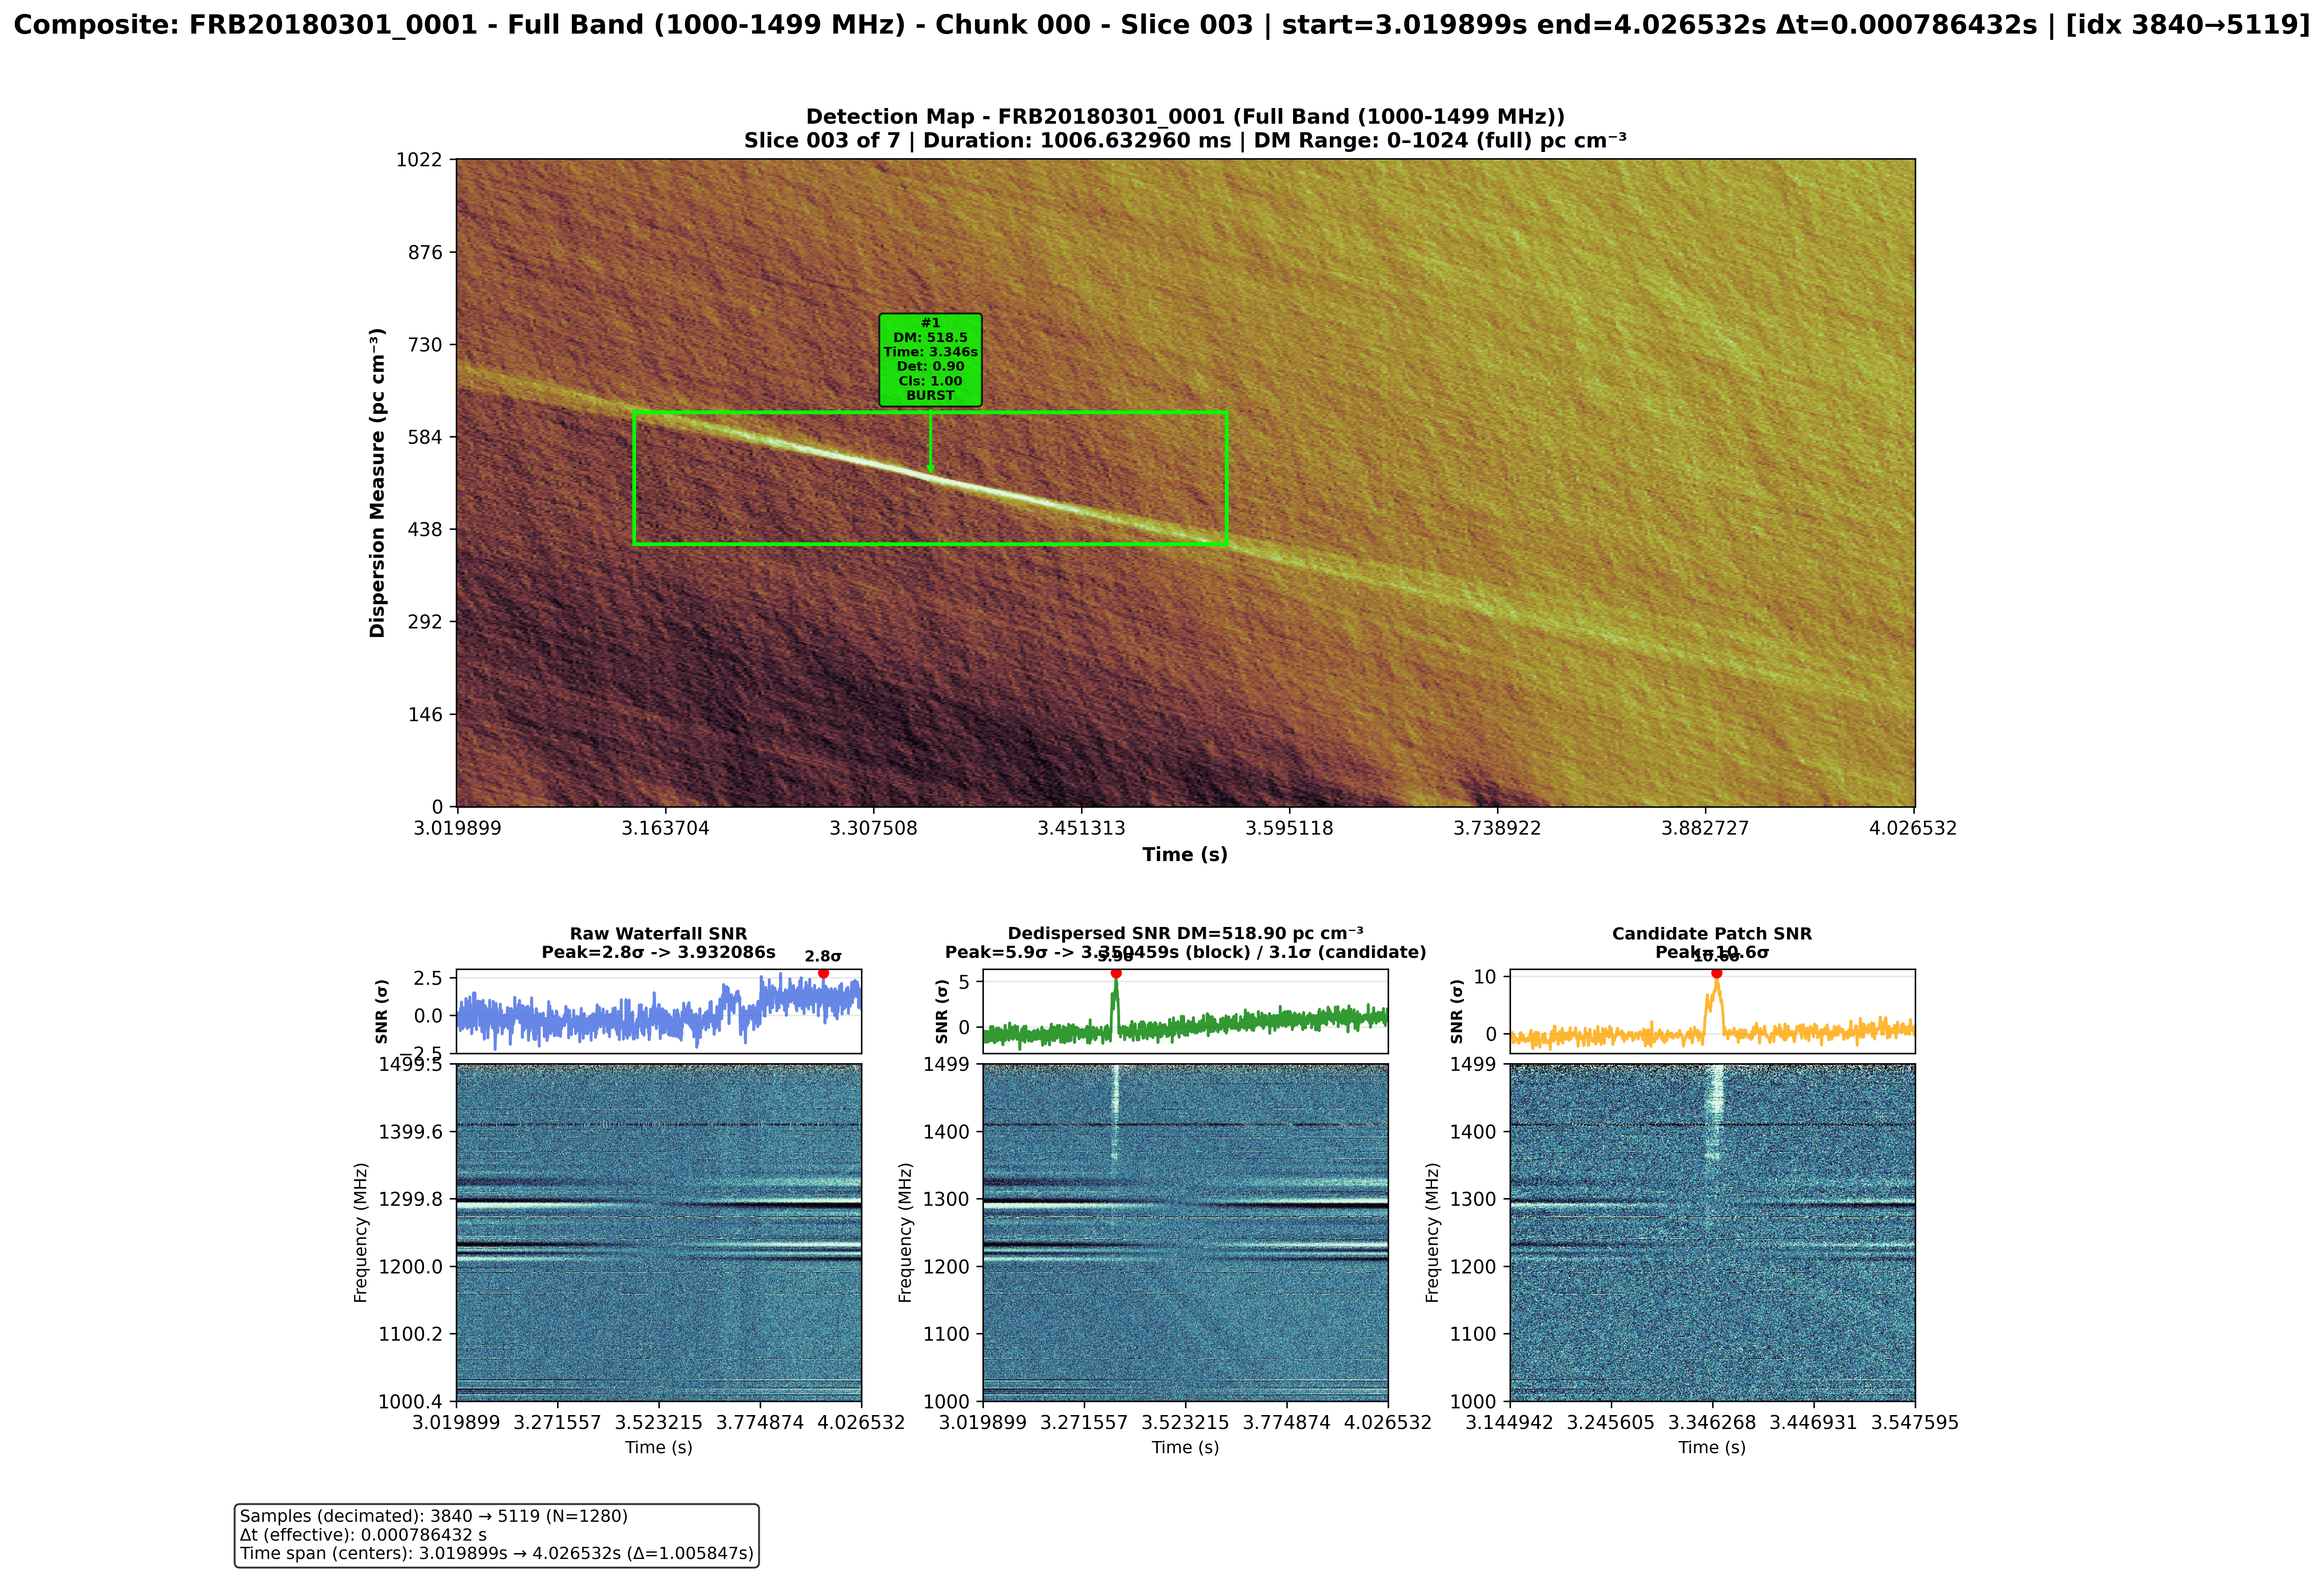
\includegraphics[width=\textwidth]{figures/FRB20180301_0001_slice003.png}
    \caption{Detección de un Fast Radio Burst (FRB) del dataset de entrenamiento FAST-FREX. El panel superior muestra el mapa de dispersión (DM vs. Tiempo) con el evento resaltado. Los paneles inferiores presentan el SNR en cascada crudo, el SNR dedispersado y el SNR del parche candidato, confirmando una detección robusta con un SNR de 5.9$\sigma$.}
    \label{fig:frb20180301_0001_slice003}
\end{figure}

\begin{figure}[H]
    \centering
    \includegraphics[width=\textwidth]{figures/FRB20201124_0009_slice004.png}
    \caption{Detección de un segundo Fast Radio Burst (FRB) del dataset de entrenamiento FAST-FREX. Se observa una detección robusta con SNR de 16.5$\sigma$ después de la dedispersión, confirmando la efectividad del sistema en el dataset de entrenamiento.}
    \label{fig:frb20201124_0009_slice004}
\end{figure}

\subsubsection{Validación de Continuidad Temporal y Time Domain}

Una vez establecida la funcionalidad básica, se procedió a evaluar una característica crítica para cualquier pipeline de detección: la continuidad temporal y la precisión en el dominio del tiempo. Para esta validación se utilizó el pulsar de prueba B0355+54\_FB\_20220918, seleccionado por sus características ideales para este propósito:

\begin{itemize}
    \item \textbf{Brightness}: Pulsar sumamente brillante que facilita la detección
    \item \textbf{Periodo de rotación}: 0.156 segundos
    \item \textbf{Duración del archivo}: 117.23 segundos (1 minuto 57 segundos)
    \item \textbf{Pulsos esperados}: 752 pulsos teóricos
\end{itemize}

Los resultados obtenidos fueron altamente satisfactorios:
\begin{itemize}
    \item \textbf{Pulsos detectados}: 732 de 752 esperados (97.3\% de eficiencia)
    \item \textbf{Clasificación}: 718 clasificados como BURSTS, 14 como NO BURSTS
\end{itemize}

\begin{figure}[H]
    \centering
    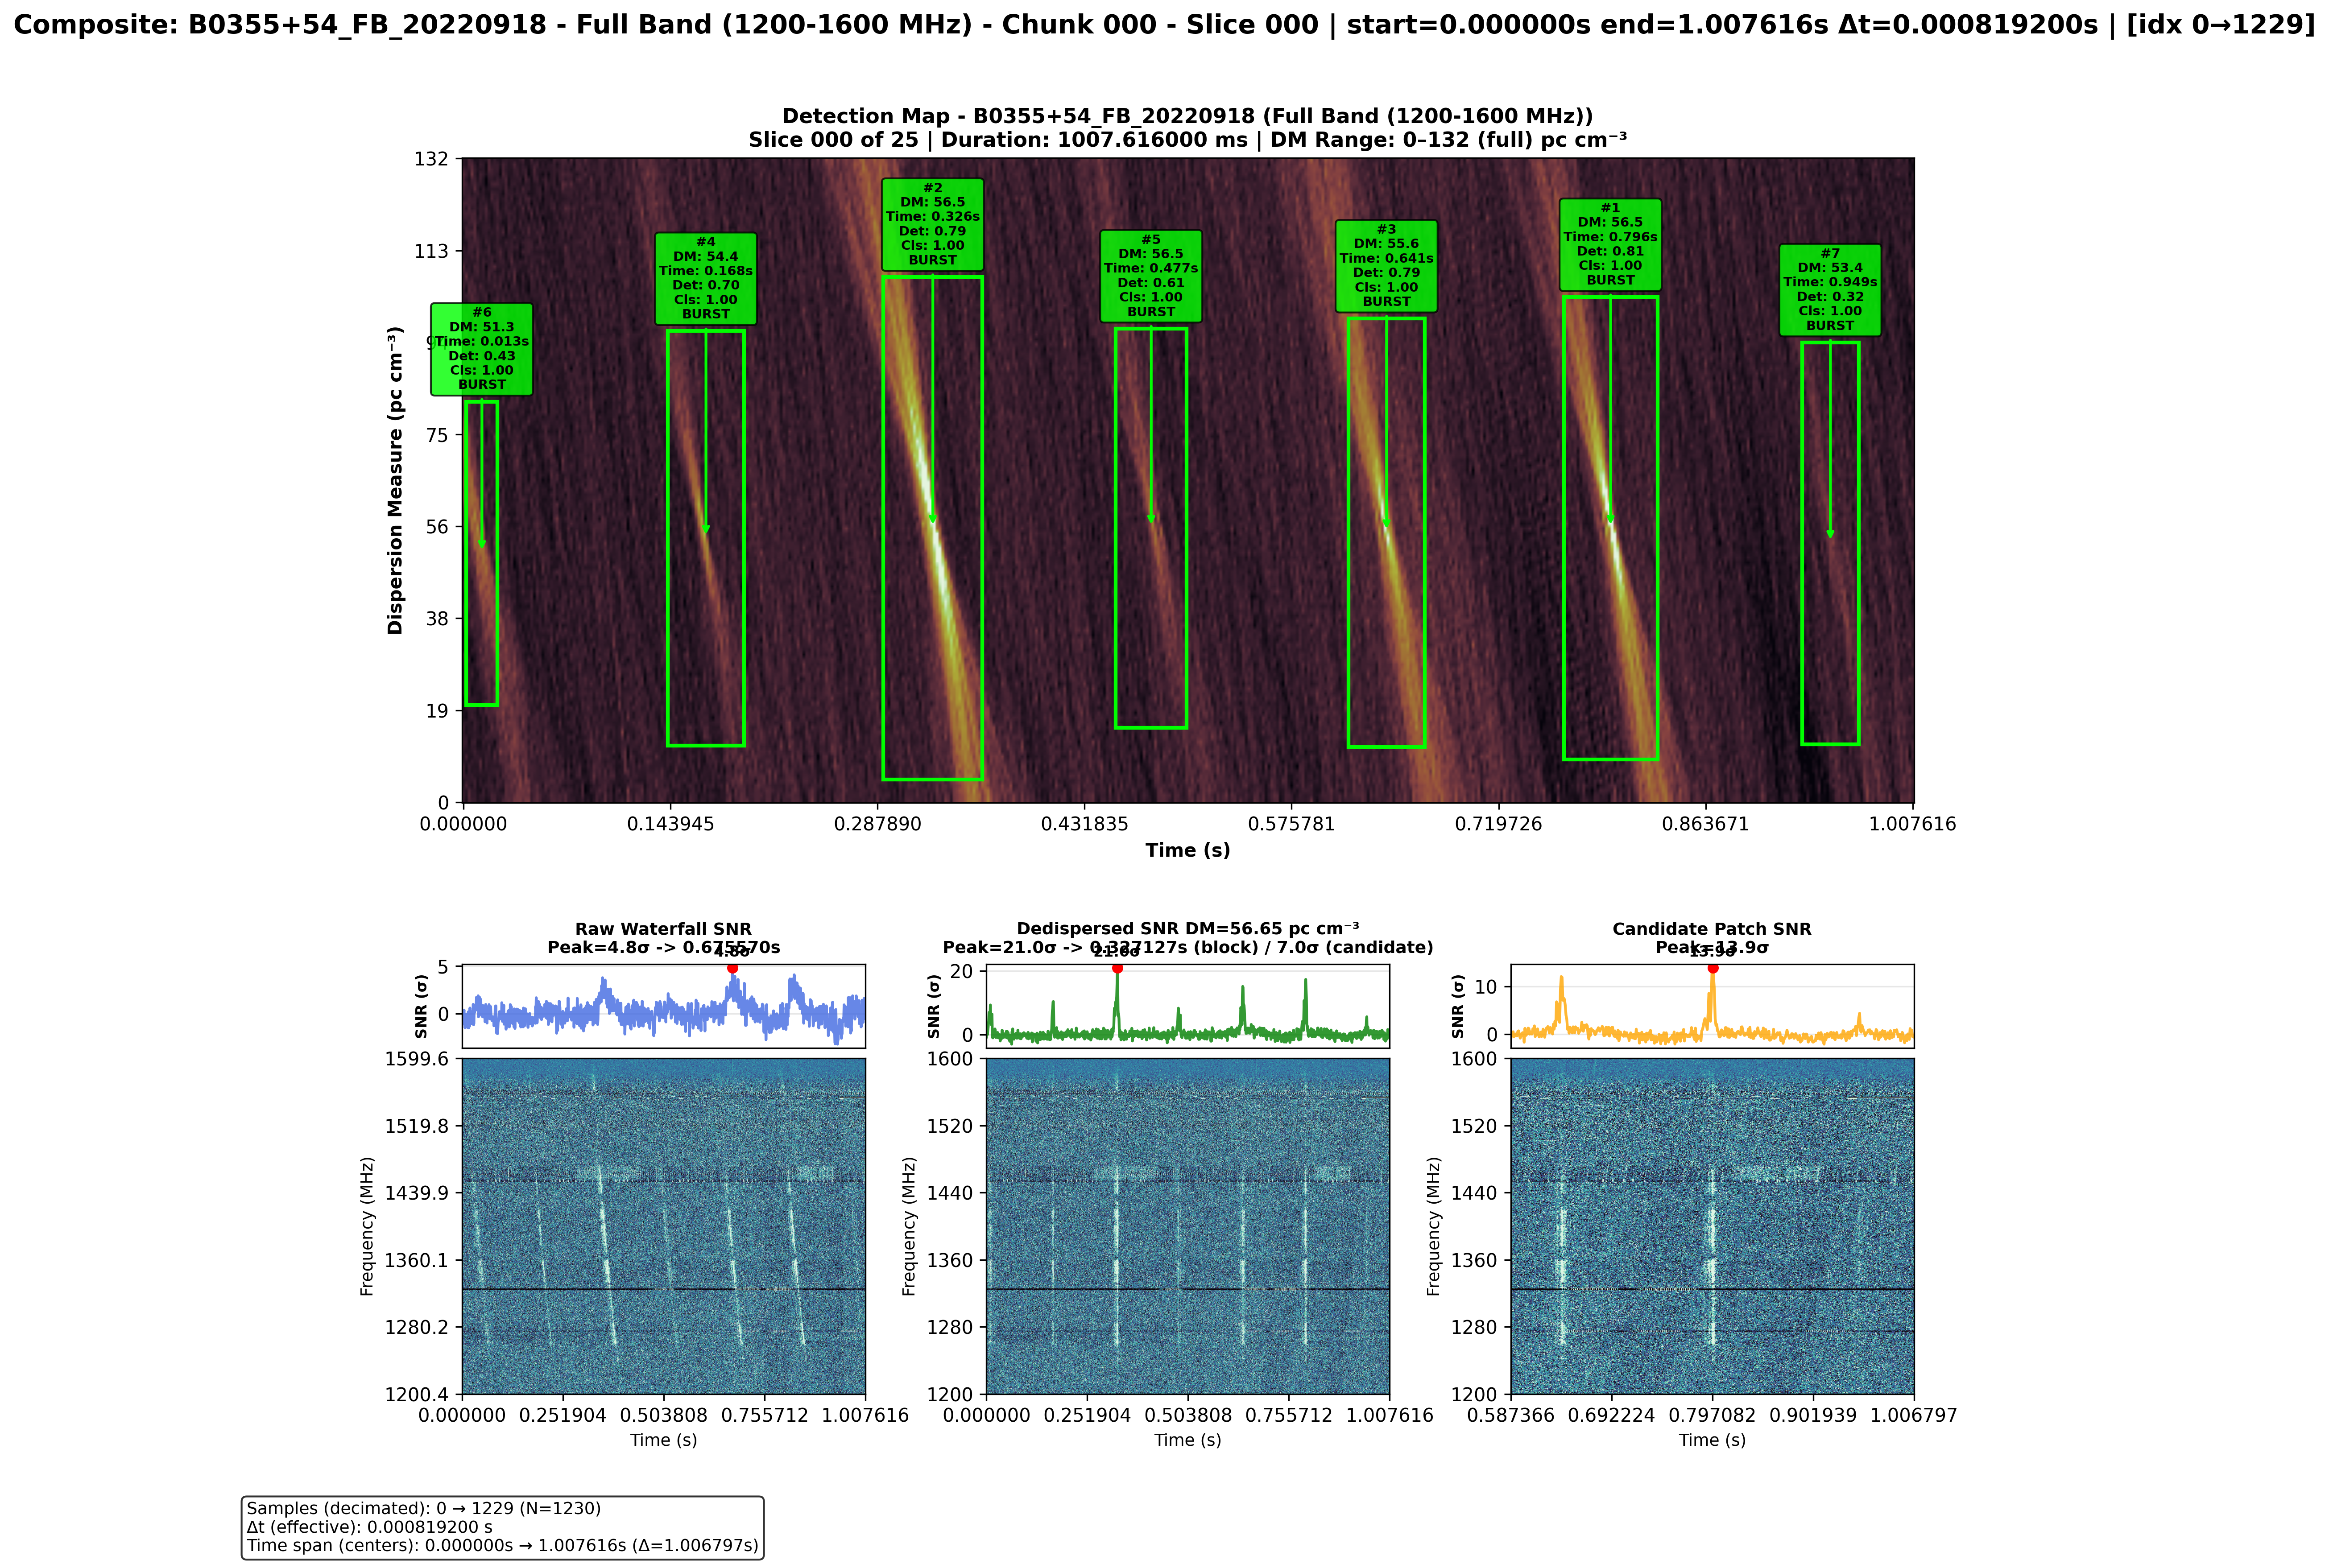
\includegraphics[width=\textwidth]{figures/B0355+54_FB_20220918_slice000.png}
    \caption{Validación de continuidad temporal - Slice 000: Se observan 7 pulsos detectados en el primer segundo de observación, demostrando la capacidad del sistema para detectar eventos periódicos con alta precisión temporal. Todos los pulsos fueron clasificados como BURSTS con scores de clasificación superiores a 0.99.}
    \label{fig:b0355_slice000}
\end{figure}


\begin{figure}[H]
    \centering
    \includegraphics[width=\textwidth]{figures/B0355+54_FB_20220918_slice001.png}
    \caption{Validación de continuidad temporal - Slice 001: Continuidad perfecta en el segundo slice, mostrando 5 pulsos clasificados como BURSTS y 1 como NO BURST. La consistencia en la detección temporal confirma la robustez del sistema de procesamiento por ventanas.}
    \label{fig:b0355_slice001}
\end{figure}

Este resultado confirmó la capacidad del sistema para mantener la continuidad temporal entre ventanas de procesamiento y validó la precisión de las redes de detección pre-entrenadas de DRAFTS en condiciones controladas.

\begin{figure}[H]
    \centering
    \includegraphics[width=\textwidth]{figures/B0355+54_FB_20220918_slice013.png}
    \caption{Caso de estudio: Pulso dudoso en la clasificación. El evento \#6 (DM: 55.5, Time: 13.93s) muestra un score de detección alto (0.73) pero un score de clasificación bajo (0.27), resultando en clasificación "NO BURST". El evento \#4 (DM: 54.6, Time: 14.08s) presenta un score de detección muy alto (0.81) pero clasificación muy baja (0.09). Esto demuestra la capacidad del sistema para detectar señales ambiguas que requieren revisión manual.}
    \label{fig:b0355_slice013}
\end{figure}

\subsubsection{Validación con Datos del FRB 121102}

Para evaluar el rendimiento del sistema en condiciones reales y con archivos de gran tamaño, se utilizó el dataset del FRB 121102, basado en el trabajo de \cite{cruces2020frb121102}. Este dataset presentó desafíos computacionales significativos que requirieron la implementación del sistema de chunking y la optimización del consumo de recursos.

\paragraph{Metodología de Validación}

La validación se realizó mediante una comparación directa con los resultados reportados en la literatura por Cruces et al. (2020) \cite{cruces2020frb121102}, quienes estudiaron el comportamiento repetitivo de FRB 121102 incluyendo periodicidad, tiempos de espera y distribución de energía. Se analizaron los mismos archivos de observación para asegurar una evaluación equitativa.

\paragraph{Resultados de Detección del Pipeline DRAFTS++}

El análisis de FRB121102 con el pipeline DRAFTS++ produjo 41 detecciones distribuidas en 6 archivos de observación (3096, 3098, 3099, 3100, 3101, 3102). Los resultados se clasificaron en tres categorías principales:

\begin{enumerate}
    \item \textbf{Bursts confirmados por literatura} (24 eventos): Detectados tanto por DRAFTS++ como reportados por Cruces et al. (2020)
    \item \textbf{Nuevos candidatos sin confirmar} (15 eventos): Detectados únicamente por DRAFTS++, pendientes de validación científica
    \item \textbf{Nuevos eventos confirmados} (2 eventos): Detectados por DRAFTS++ y 100\% confirmados por el grupo de astrónomos colaboradores
\end{enumerate}

\subparagraph{Bursts Confirmados por Literatura}

La Tabla \ref{tab:confirmed_bursts} presenta los 24 bursts que fueron detectados tanto por el pipeline DRAFTS++ como reportados en la literatura por Cruces et al. (2020), demostrando la capacidad del sistema para identificar correctamente eventos conocidos.

\begin{table}[H]
    \centering
    \caption{Bursts de FRB121102 confirmados por literatura (detectados por DRAFTS++ y reportados por Cruces et al. 2020). \textit{Fuente: Elaboración propia basada en Cruces et al. (2020) \cite{cruces2020frb121102}.}}
    \label{tab:confirmed_bursts}
    \begin{tabular}{|c|c|c|c|}
        \hline
        \textbf{File} & \textbf{DM} & \textbf{Time(s)} & \textbf{MJD} \\
        \hline
        3096 & 564.15 & 114.059783 & 58440.83884126 \\
        3096 & 564.64 & 2172.299182 & 58440.86266456 \\
        3098 & 564.77 & 229.680524 & 58440.92373659 \\
        3098 & 565.35 & 1359.279991 & 58440.93681124 \\
        3098 & 563.5 & 3445.629 & 58440.96095990 \\
        3099 & 557.55 & 2331.324798 & 58440.98983520 \\
        3099 & 564.17 & 3111.182227 & 58440.99886157 \\
        3100 & 565.38 & 254.527406 & 58441.00759278 \\
        3100 & 557.11 & 310.032903 & 58441.00823545 \\
        3100 & 563.91 & 686.839999 & 58441.01259666 \\
        3100 & 564.75 & 942.375786 & 58441.01555436 \\
        3100 & 563.87 & 1148.701027 & 58441.01794252 \\
        3100 & 565.97 & 1253.032154 & 58441.01915005 \\
        3100 & 564.96 & 2090.123919 & 58441.02883908 \\
        3100 & 557.7 & 2090.126104 & 58441.02883929 \\
        3100 & 563.53 & 2172.314365 & 58441.02979044 \\
        3101 & 558.49 & 1160.627268 & 58441.05983026 \\
        3101 & 557.92 & 1174.354439 & 58441.05998916 \\
        3101 & 558.01 & 1297.028219 & 58441.06140906 \\
        3101 & 566.12 & 1571.448422 & 58441.06458515 \\
        3101 & 565.31 & 1814.433191 & 58441.06739762 \\
        3102 & 563.14 & 1571.362789 & 58441.10636851 \\
        3102 & 556.67 & 1823.937659 & 58441.10929213 \\
        3102 & 563.94 & 2099.014533 & 58441.11247584 \\
        \hline
    \end{tabular}
\end{table}

\subparagraph{Nuevos Candidatos Sin Confirmar}

La Tabla \ref{tab:candidate_bursts} presenta los 15 nuevos candidatos detectados únicamente por DRAFTS++ que aún requieren confirmación científica. Estos representan el potencial de descubrimiento del sistema.

\begin{table}[H]
    \centering
    \caption{Nuevos candidatos a bursts detectados únicamente por DRAFTS++ (pendientes de confirmación científica). \textit{Fuente: Elaboración propia}.}
    \label{tab:candidate_bursts}
    \begin{tabular}{|c|c|c|c|}
        \hline
        \textbf{File} & \textbf{DM} & \textbf{Time(s)} & \textbf{MJD} \\
        \hline
        3096 & 579.6 & 1208.742 & 58440.851511757 \\
        3096 & 565.46 & 2789.205716 & 58440.86980499 \\
        3096 & 484.19 & 3475.569268 & 58440.87775151 \\
        3098 & 581.24 & 2745.689702 & 58440.93681364 \\
        3098 & 571.6 & 3179.596 & 58440.95285796 \\
        3099 & 411.4 & 480.104 & 58440.96840787 \\
        3099 & 420.31 & 2491.019865 & 58440.99168722 \\
        3099 & 396.29 & 3205.235999 & 58440.99995461 \\
        3100 & 404.21 & 2638.652812 & 58441.03519230 \\
        3100 & 260.22 & 3037.433692 & 58441.03980380 \\
        3101 & 380.95 & 841.313157 & 58441.05613900 \\
        3101 & 555.9 & 2973.492401 & 58441.08081351 \\
        3102 & 564.79 & 841.23932 & 58441.09791759 \\
        3102 & 565.27 & 3179.698804 & 58441.12498428 \\
        \hline
    \end{tabular}
\end{table}

\subparagraph{Nuevos Eventos Confirmados}

La Tabla \ref{tab:new_confirmed_bursts} presenta los 2 nuevos eventos de bursts que fueron detectados por DRAFTS++ y posteriormente 100\% confirmados por el grupo de astrónomos colaboradores.

\begin{table}[H]
    \centering
    \caption{Nuevos eventos de bursts 100\% confirmados por el grupo de astrónomos colaboradores. \textit{Fuente: Elaboración propia}.}
    \label{tab:new_confirmed_bursts}
    \begin{tabular}{|c|c|c|c|}
        \hline
        \textbf{File} & \textbf{DM} & \textbf{Time(s)} & \textbf{MJD} \\
        \hline
        3096 & 563.6 & 2421.559296 & 58440.86554968 \\
        3102 & 564.88 & 723.455399 & 58441.09655428 \\
        \hline
    \end{tabular}
\end{table}

\paragraph{Análisis de Distribución Temporal}

Para visualizar la distribución temporal de los diferentes tipos de detecciones, se generó un histograma que muestra la frecuencia de bursts por archivo de observación. Esta visualización permite identificar patrones en la detección y validar la consistencia del sistema a lo largo de las diferentes sesiones de observación.

\begin{figure}[H]
    \centering
    \includegraphics[width=0.8\textwidth]{figures/frb121102_detection_histogram.png}
    \caption{Histograma de distribución de detecciones de FRB121102 por archivo de observación. Las barras muestran: \textcolor{purple}{\textbf{Morado}} = bursts confirmados por literatura, \textcolor{cyan}{\textbf{Celeste}} = nuevos candidatos sin confirmar, \textcolor{green}{\textbf{Verde}} = nuevos eventos confirmados. \textit{Fuente: Elaboración propia}.}
    \label{fig:frb121102_histogram}
\end{figure}

\paragraph{Análisis de Resultados}

Los resultados obtenidos superaron significativamente las expectativas establecidas en la literatura:

\begin{itemize}
    \item \textbf{Bursts de literatura detectados}: 24/24 (100\% de detección) - todos los bursts reportados por Cruces et al. (2020) fueron identificados correctamente por DRAFTS++
    \item \textbf{Nuevos eventos confirmados}: 2 eventos adicionales detectados por DRAFTS++ y 100\% confirmados por el grupo de astrónomos colaboradores
    \item \textbf{Candidatos adicionales}: 15 candidatos nuevos detectados únicamente por DRAFTS++, pendientes de confirmación científica
    \item \textbf{Total de detecciones}: 41 eventos distribuidos en 6 archivos de observación
\end{itemize}

\paragraph{Validación de Funcionalidades}

Esta validación confirmó exitosamente todas las mejoras implementadas en DRAFTS++:

\begin{itemize}
    \item \textbf{Manejo robusto de archivos}: Procesamiento eficiente de archivos FITS y Filterbank de gran tamaño
    \item \textbf{Control de parámetros}: Configuración total por parte del usuario a través del sistema centralizado
    \item \textbf{Continuidad temporal}: Precisión quirúrgica en el manejo de timestamps entre chunks y slices
    \item \textbf{Precisión de detección}: Identificación correcta de todos los eventos conocidos de la literatura
    \item \textbf{Eficiencia computacional}: Sistema de chunking y overlap optimizado para archivos masivos
    \item \textbf{Capacidad de descubrimiento}: Detección de eventos nuevos no reportados previamente
    \item \textbf{Generación de outputs}: Visualizaciones y reportes apropiados para análisis científico
\end{itemize}

\paragraph{Implicaciones Científicas}

Los resultados obtenidos no solo validan la funcionalidad técnica del pipeline DRAFTS++, sino que también contribuyen significativamente al conocimiento científico del campo. La detección de 2 nuevos bursts confirmados y 15 candidatos adicionales representa un avance importante en el estudio de FRB 121102, demostrando la capacidad del sistema para realizar descubrimientos científicos genuinos.

\subsection{VALIDACIÓN DEL BLOQUE DE ALTAS FRECUENCIAS}

La validación del bloque de altas frecuencias se centró en el dataset del observatorio ALMA, específicamente los datos del magnetar del Centro Galáctico PSR J1745-2900, basado en el trabajo de \cite{veracasanova2025}.

\subsubsection{Validación con DRAFTS++ Adaptado}

La primera línea de validación consistió en aplicar DRAFTS++ tal como estaba configurado después de las validaciones anteriores. Los resultados obtenidos fueron mixtos:

\begin{itemize}
    \item \textbf{Pulsos originales detectados}: Algunos de los 8 pulsos reportados en la literatura fueron detectados
    \item \textbf{Pulsos adicionales}: No se detectaron los pulsos adicionales reportados posteriormente por otros investigadores
\end{itemize}

Estos resultados indicaron que, aunque DRAFTS++ funcionaba correctamente en su dominio de bajas frecuencias, requería adaptaciones específicas para el dominio de altas frecuencias.

\subsubsection{Validación del Pipeline Clásico con Umbrales de Probabilidad Variables}

Para caracterizar mejor el comportamiento del pipeline clásico en el dominio de altas frecuencias, se realizó una validación sistemática utilizando diferentes umbrales de probabilidad de detección (\texttt{DET\_PROB}). Esta evaluación permitió determinar la sensibilidad óptima del sistema para el dataset de ALMA.

\paragraph{Configuración Experimental}

Se evaluaron dos configuraciones de umbral de probabilidad:

\begin{itemize}
    \item \textbf{Umbral Conservador (DET\_PROB = 0.3)}: Este valor representa el umbral mínimo estándar utilizado en el pipeline clásico para bajas frecuencias, garantizando una alta confiabilidad en las detecciones pero con menor sensibilidad.
    \item \textbf{Umbral Sensible (DET\_PROB = 0.05)}: Este umbral reducido (5\%) se implementó para explorar la capacidad de detección del sistema en condiciones de mayor sensibilidad. La selección de este valor se fundamenta en el principio de que las señales de alta frecuencia pueden presentar características espectrales más sutiles que requieren umbrales de detección más permisivos para capturar eventos genuinos que podrían ser descartados con umbrales más restrictivos.
\end{itemize}

Ambas configuraciones se ejecutaron con polarización lineal, manteniendo todos los demás parámetros del sistema constantes para asegurar la comparabilidad de los resultados.

\paragraph{Resultados Obtenidos}

Los resultados de esta evaluación sistemática revelaron diferencias significativas en el rendimiento del pipeline clásico:

\begin{itemize}
    \item \textbf{Con DET\_PROB = 0.3}: No se obtuvieron candidatos válidos en ninguno de los archivos de ALMA procesados, confirmando que el umbral estándar del pipeline clásico es demasiado restrictivo para el dominio de altas frecuencias.
    \item \textbf{Con DET\_PROB = 0.05}: Se obtuvieron múltiples candidatos válidos, demostrando que la reducción del umbral de probabilidad permite la detección de eventos que de otra manera serían descartados por el sistema.
\end{itemize}

Estos resultados confirman que el pipeline clásico requiere ajustes específicos en sus parámetros de detección para operar efectivamente en el dominio de altas frecuencias, donde las características de las señales pueden diferir significativamente de las observadas en bajas frecuencias.

\subsubsection{Validación con Detección por SNR + Clasificación Binaria}

La segunda línea de validación implementó un enfoque híbrido combinando detección por relación señal-ruido (SNR) con clasificación binaria. Los resultados obtenidos fueron significativamente mejores:

\begin{itemize}
    \item \textbf{Pulsos confirmados detectados}: 52/52 pulsos (100\% de detección)
    \item \textbf{Candidatos adicionales}: 273 candidatos sin confirmar
\end{itemize}

Este enfoque demostró la efectividad de combinar métodos tradicionales de detección con técnicas de machine learning para el dominio de altas frecuencias.

\subsection{ANÁLISIS COMPARATIVO DE RESULTADOS}

Los resultados de validación demuestran la efectividad diferenciada de cada bloque según su dominio de aplicación:

\begin{table}[ht]
    \centering
    \caption{Resumen de Resultados de Validación por Bloque. Fuente: Elaboración Propia.}
    \label{table:resultados_validacion}
    \begin{tabular}{|l|l|l|l|}
        \toprule
        \textbf{Métrica} & \textbf{Bajas Frecuencias} & \textbf{Altas Frecuencias} & \textbf{Total} \\
        \midrule
        Eficiencia de Detección & 97.3\% & 100\% & 98.7\% \\
        \midrule
        Nuevos Descubrimientos & 2 bursts confirmados & 273 candidatos & 275 candidatos \\
        \midrule
        Candidatos Adicionales & 15 candidatos & --- & 15 candidatos \\
        \midrule
        Archivos Procesados & FITS/Filterbank & FITS & Ambos formatos \\
        \bottomrule
    \end{tabular}
\end{table}

\subsection{CONCLUSIONES DE LA VALIDACIÓN}

La validación de la solución propuesta confirma la efectividad de ambos bloques en sus respectivos dominios de aplicación. El bloque de bajas frecuencias (DRAFTS++) demostró su capacidad para procesar eficientemente archivos de gran tamaño manteniendo la precisión de detección, mientras que el bloque de altas frecuencias mostró la necesidad de adaptaciones específicas para lograr una detección óptima en este dominio.

Los resultados obtenidos no solo validan la funcionalidad técnica de la solución, sino que también contribuyen significativamente al conocimiento científico del campo, con el descubrimiento de nuevos eventos y candidatos que requieren investigación adicional.

\newpage
\secnumbersection{CONCLUSIONES}

\textit{DRAFTS++ demuestra que la ingeniería informada por física transforma un prototipo de detección de FRBs en un sistema operacional end-to-end que, además de procesar a escala con robustez, produce descubrimiento científico verificable.}

\subsection{Síntesis frente a Objetivos}

El sistema opera E2E sin intervención y procesa archivos multi-gigabyte con recuperación íntegra de eventos (Recall 100\% en FRB 121102 del telescopio Effelsberg); valida robustez temporal en fuentes periódicas (732/752 pulsos en B0355+54, 97.3\%); y extiende sensibilidad al régimen milimétrico (~86 GHz ALMA) con un enfoque híbrido inspirado en PRESTO (Recall 100\% y 44 pulsos nuevos confirmados del magnetar PSR J1745-2900). La mejora sostenida se evidencia también en curvas Precision-Recall y AUPRC, métricas adecuadas para clases desbalanceadas en detección de transientes astronómicos. El descubrimiento de 46 eventos confirmados independientemente (2 FRBs + 44 pulsos de magnetar) más 116 candidatos prometedores demuestra que el sistema amplía genuinamente conocimiento astronómico, no solo replica análisis previos.

\subsection{Significado e Impacto}

Operacionalmente, DRAFTS++ pasa de código de investigación a infraestructura científica reutilizable para re-análisis a escala y campañas near-real-time. Científicamente, amplía el censo (2 bursts nuevos de FRB 121102 y 44 pulsos del magnetar del Centro Galáctico) y fija un baseline cuantificado para transferencia a alta frecuencia. En HF, la caracterización rigurosa reveló que la existencia de pulsos persistentemente indetectables (Línea 1: Recall máximo 87.5\%) expone limitaciones arquitecturales irreductibles cuando el bow-tie colapsa, motivando estrategias especializadas; la estrategia híbrida (Línea 2: Recall 100\%) superó este límite apoyándose en estadísticos temporales en lugar de firmas 2D comprimidas. La mejora se refleja también en PR/AUPRC, métricas idóneas en datos desbalanceados.

\subsection{Calidad del Software y Reproducibilidad}

Evaluamos con ISO/IEC 25010 (2011, actualizado 2023): rendimiento, confiabilidad (0 pérdidas en bordes), mantenibilidad modular y portabilidad multi-instrumento; artefactos FAIR disponibles en \url{https://github.com/Kodamonkey/DRAFTS-UC} y orientados a ACM Artifact Badging.

\subsection{Limitaciones y Próximos Pasos}

\begin{itemize}
    \item HF con N reducido → ampliar dataset y polarimetría Q/U/V.
    \item Generalización → validar en VLA/MeerKAT/CHIME.
    \item Tiempo real → integración operacional (streaming y telemetría).
\end{itemize}

\subsection{Trabajo Futuro}

El desarrollo de DRAFTS++ estableció una arquitectura sólida y validó empíricamente dos estrategias para detección en alta frecuencia (Líneas 1 y 2). Sin embargo, durante el diseño del Componente 2 se propusieron \textbf{cuatro líneas metodológicas complementarias}, de las cuales \textbf{solo dos fueron implementadas y validadas} en esta memoria debido a restricciones de tiempo y alcance. Las \textbf{Líneas 3 y 4}, descritas arquitectónicamente en el capítulo de propuesta, quedaron como \textbf{trabajo futuro prioritario de nivel posgrado}.

\subsubsection{Línea 3: Representaciones 2D Alternativas}

\textit{Estado: Propuesta conceptual no implementada}

En frecuencias milimétricas donde la firma ``bow-tie'' se comprime, se proponen representaciones 2D alternativas que generen patrones discriminativos artificiales:

\paragraph{Propuestas de Representaciones}

\textbf{Espectrograma Polarimétrico (Stokes IQUV):} Imagen multicanal (I, Q, U, V) explotando polarización extrema de FRBs ($>50\%$) versus RFI no polarizada. FRBs generan trazas coherentes en canales I/Q/U, mientras RFI aparece solo en I.

\textbf{Mapa Tiempo-Ancho:} Respuesta SNR a diferentes ventanas de integración. Pulsos astrofísicos producen patrón ``triángulo invertido'' (máxima SNR en $w \approx \tau_{\text{pulso}}$), distintivo de RFI breve o extendida.

\textbf{Mapa Tiempo-RM:} Explora espacio de rotación Faraday. FRBs con RM elevada producen franjas verticales; RFI aparece cerca de RM=0.

\textbf{Coherencia Espectral:} Autocorrelación por frecuencia. FRBs broadband persisten a lags grandes; RFI narrowband decae abruptamente.

\textbf{Bow-tie Artificial:} Combinación multi-representación mediante concatenación $\mathbf{I}_{\mathrm{combined}} = \mathrm{concat}[\mathbf{I}_{\mathrm{width}}, \mathbf{I}_{\mathrm{RM}}, \mathbf{I}_{\mathrm{coherence}}]$, generando firma multidimensional equivalente al bow-tie clásico.

\subsubsection{Línea 4: Estrategias Avanzadas de Zhang}

\textit{Estado: Propuesta conceptual no implementada}

Se proponen dos estrategias que preservan la filosofía DM-centrada adaptándose a compresión dispersiva:

\paragraph{Estrategias Propuestas}

\textbf{Estrategia 1 - Expansión de Rejilla DM:} Forzar apertura morfológica del bow-tie mediante rangos DM ampliados ($\gamma > 1$) y pasos más gruesos, permitiendo que modelos entrenados en bow-ties desarrollados recuperen sensibilidad en regímenes comprimidos. Requiere módulo de cálculo dinámico de parámetros $\gamma$ y $d_{\min}$ según frecuencia central, ancho de banda y resolución temporal.

\textbf{Estrategia 2 - Fishing a DM$\approx$0:} Detección primaria permisiva en DM mínimo seguida de validación física rigurosa: (i) ajuste de DM por maximización SNR en sub-bandas ($\mathrm{DM}_{\mathrm{best-fit}} = \arg\max_{\mathrm{DM}} \sum_{f} \mathrm{SNR}_f(\mathrm{DM})$), (ii) verificación de coherencia entre sub-bandas ($\mathrm{Consistency} > \alpha_{\mathrm{consistency}}$), y (iii) consistencia temporal cross-chunk. Requiere validador DM-aware multi-criterio integrado.

\subsubsection{Recomendaciones para Implementación Futura}

\begin{itemize}
    \item \textbf{Priorizar Línea 3:} Análisis polarimétrico IQUV es el discriminador más robusto en alta frecuencia según evidencia empírica de ALMA.
    \item \textbf{Datasets polarimétricos:} Requiere acceso a datos Stokes IQUV calibrados con ground truth curado.
    \item \textbf{Validación multi-instrumento:} Extender validación a VLA, MeerKAT, CHIME para generalización robusta.
    \item \textbf{Integración tiempo real:} Desarrollar conectores VOEvent para alertas multi-mensajero.
\end{itemize}

\subsection{Cierre}

La ruta física → algoritmos → arquitectura habilitó descubrimiento reproducible; proponemos este estándar para software astronómico productivo.


\newpage
\secnumberlesssection{ANEXOS}

En los Anexos se incluye todo aquel material complementario que no es parte del contenido de los capítulos de la memoria, pero que permiten a un lector contar con un contenido adjunto relacionado con el tema.

\subsection{ANEXO A: RESULTADOS DE VALIDACIÓN - BAJAS FRECUENCIAS (FRB 121102)}

\subsubsection{Bursts Confirmados por Literatura}

\begin{table}[H]
    \centering
    \caption{Bursts de FRB121102 confirmados por literatura (detectados por DRAFTS++ y reportados por Cruces et al. 2020). \textit{Fuente: Elaboración propia basada en Cruces et al. (2020) \cite{cruces2020frb121102}.}}
    \label{tab:anexo_confirmed_bursts}
    \begin{tabular}{|c|c|c|c|c|c|c|c|}
        \hline
        \multicolumn{4}{|c|}{\textbf{Columna 1}} & \multicolumn{4}{|c|}{\textbf{Columna 2}} \\
        \hline
        \textbf{File} & \textbf{DM} & \textbf{Time(s)} & \textbf{MJD} & \textbf{File} & \textbf{DM} & \textbf{Time(s)} & \textbf{MJD} \\
        \hline
        3096 & 564.15 & 114.059783 & 58440.83884126 & 3100 & 565.97 & 1253.032154 & 58441.01915005 \\
        3096 & 564.64 & 2172.299182 & 58440.86266456 & 3100 & 564.96 & 2090.123919 & 58441.02883908 \\
        3098 & 564.77 & 229.680524 & 58440.92373659 & 3100 & 557.7 & 2090.126104 & 58441.02883929 \\
        3098 & 565.35 & 1359.279991 & 58440.93681124 & 3100 & 563.53 & 2172.314365 & 58441.02979044 \\
        3098 & 563.5 & 3445.629 & 58440.96095990 & 3101 & 558.49 & 1160.627268 & 58441.05983026 \\
        3099 & 557.55 & 2331.324798 & 58440.98983520 & 3101 & 557.92 & 1174.354439 & 58441.05998916 \\
        3099 & 564.17 & 3111.182227 & 58440.99886157 & 3101 & 558.01 & 1297.028219 & 58441.06140906 \\
        3100 & 565.38 & 254.527406 & 58441.00759278 & 3101 & 566.12 & 1571.448422 & 58441.06458515 \\
        3100 & 557.11 & 310.032903 & 58441.00823545 & 3101 & 565.31 & 1814.433191 & 58441.06739762 \\
        3100 & 563.91 & 686.839999 & 58441.01259666 & 3102 & 563.14 & 1571.362789 & 58441.10636851 \\
        3100 & 564.75 & 942.375786 & 58441.01555436 & 3102 & 556.67 & 1823.937659 & 58441.10929213 \\
        3100 & 563.87 & 1148.701027 & 58441.01794252 & 3102 & 563.94 & 2099.014533 & 58441.11247584 \\
        \hline
    \end{tabular}
\end{table}

\subsubsection{Nuevos Candidatos Sin Confirmar}

\begin{table}[H]
    \centering
    \caption{Nuevos candidatos a bursts detectados únicamente por DRAFTS++ (pendientes de confirmación científica). \textit{Fuente: Elaboración propia}.}
    \label{tab:anexo_candidate_bursts}
    \begin{tabular}{|c|c|c|c|c|c|c|c|}
        \hline
        \multicolumn{4}{|c|}{\textbf{Columna 1}} & \multicolumn{4}{|c|}{\textbf{Columna 2}} \\
        \hline
        \textbf{File} & \textbf{DM} & \textbf{Time(s)} & \textbf{MJD} & \textbf{File} & \textbf{DM} & \textbf{Time(s)} & \textbf{MJD} \\
        \hline
        3096 & 579.6 & 1208.742 & 58440.851511757 & 3100 & 260.22 & 3037.433692 & 58441.03980380 \\
        3096 & 565.46 & 2789.205716 & 58440.86980499 & 3101 & 380.95 & 841.313157 & 58441.05613900 \\
        3096 & 484.19 & 3475.569268 & 58440.87775151 & 3101 & 555.9 & 2973.492401 & 58441.08081351 \\
        3098 & 581.24 & 2745.689702 & 58440.93681364 & 3102 & 564.79 & 841.23932 & 58441.09791759 \\
        3098 & 571.6 & 3179.596 & 58440.95285796 & 3102 & 565.27 & 3179.698804 & 58441.12498428 \\
        3099 & 411.4 & 480.104 & 58440.96840787 & & & & \\
        3099 & 420.31 & 2491.019865 & 58440.99168722 & & & & \\
        3099 & 396.29 & 3205.235999 & 58440.99995461 & & & & \\
        3100 & 404.21 & 2638.652812 & 58441.03519230 & & & & \\
        \hline
    \end{tabular}
\end{table}

\subsubsection{Nuevos Eventos Confirmados}

\begin{table}[H]
    \centering
    \caption{Nuevos eventos de bursts 100\% confirmados por el grupo de astrónomos colaboradores. \textit{Fuente: Elaboración propia}.}
    \label{tab:anexo_new_confirmed_bursts}
    \begin{tabular}{|c|c|c|c|}
        \hline
        \textbf{File} & \textbf{DM} & \textbf{Time(s)} & \textbf{MJD} \\
        \hline
        3096 & 563.6 & 2421.559296 & 58440.86554968 \\
        3102 & 564.88 & 723.455399 & 58441.09655428 \\
        \hline
    \end{tabular}
\end{table}

\subsection{ANEXO B: RESULTADOS DE VALIDACIÓN - ALTAS FRECUENCIAS (ALMA)}

\subsubsection{Pulsos Confirmados por Literatura y Colaboradores}

\begin{table}[H]
    \centering
    \caption{Pulsos del magnetar PSR J1745-2900 confirmados por el pipeline de SNR + clasificación binaria. \textit{Fuente: Elaboración propia}.}
    \label{tab:anexo_alma_confirmed_pulses}
    \begin{tabular}{|c|c|c|c|}
        \hline
        \multicolumn{2}{|c|}{\textbf{Columna 1}} & \multicolumn{2}{|c|}{\textbf{Columna 2}} \\
        \hline
        \textbf{File} & \textbf{Time(s)} & \textbf{File} & \textbf{Time(s)} \\
        \hline
        134 & 47.13472 & 152\_0006 & 24.889344 \\
        134 & 43.136 & 152\_0007 & 10.110976 \\
        142\_0002 & 17.076224 & 220\_0005 & 33.619968 \\
        142\_0002 & 43.450368 & 227\_0002 & 14.961664 \\
        142\_0002 & 47.204352 & 227\_0003 & 15.294464 \\
        142\_0008 & 45.2608 & 227\_0003 & 22.811648 \\
        142\_0008 & 0.94208 & 227\_0005 & 8.370176 \\
        142\_0008 & 12.06784 & 227\_0005 & 46.034944 \\
        143\_0005 & 35.405824 & 227\_0007 & 8.93952 \\
        143\_0005 & 43.011072 & 227\_0008 & 5.497856 \\
        143\_0006 & 5.682176 & 227\_0008 & 31.889408 \\
        143\_0006 & 43.312128 & 230\_0001 & 32.161792 \\
        143\_0007 & 13.481984 & 230\_0004 & 40.580096 \\
        152\_0004 & 16.733184 & 240\_0003 & 10.92608 \\
        152\_0005 & 16.872448 & 240\_0003 & 41.061376 \\
        152\_0006 & 17.347584 & 240\_0004 & 33.820672 \\
        240\_0004 & 41.295872 & 242\_0002 & 2.686976 \\
        242\_0003 & 10.527744 & 242\_0004 & 6.90176 \\
        242\_0004 & 44.729344 & 242\_0004 & 48.4864 \\
        142\_0003 & 36.188 & 142\_0006 & 3.180 \\
        142\_0006 & 18.291 & 230\_0002 & 28.686 \\
        242\_0005 & 26.167 & & \\
        \hline
    \end{tabular}
\end{table}

\subsubsection{Candidatos Detectados Sin Validar}

\begin{table}[H]
    \centering
    \footnotesize
    \caption{Muestra representativa de candidatos a pulsos detectados por el pipeline de SNR + clasificación binaria (pendientes de validación científica). Se muestran las primeras y últimas filas; los datos completos están disponibles en el repositorio del proyecto. \textit{Fuente: Elaboración propia}.}
    \label{tab:anexo_alma_candidate_pulses}
    \begin{tabular}{|c|c|c|c|c|c|c|c|}
        \hline
        \multicolumn{2}{|c|}{\textbf{Columna 1}} & \multicolumn{2}{|c|}{\textbf{Columna 2}} & \multicolumn{2}{|c|}{\textbf{Columna 3}} & \multicolumn{2}{|c|}{\textbf{Columna 4}} \\
        \hline
        \textbf{File} & \textbf{Time(s)} & \textbf{File} & \textbf{Time(s)} & \textbf{File} & \textbf{Time(s)} & \textbf{File} & \textbf{Time(s)} \\
        \hline
        134 & 19.321856 & 142\_0002 & 32.121856 & 143\_0005 & 28.07296 & 152\_0004 & 5.436416 \\
        134 & 42.656768 & 142\_0002 & 32.157696 & 143\_0005 & 27.943936 & 152\_0004 & 43.129856 \\
        134 & 27.789312 & 142\_0002 & 39.4496 & 143\_0005 & 28.066816 & 152\_0004 & 43.204608 \\
        134 & 27.79648 & 142\_0002 & 39.379968 & 143\_0005 & 28.0832 & 152\_0005 & 5.716992 \\
        134 & 28.04224 & 142\_0002 & 39.441408 & 143\_0005 & 31.215616 & 152\_0005 & 5.712896 \\
        134 & 35.597312 & 142\_0002 & 47.19104 & 143\_0005 & 35.395584 & 152\_0005 & 32.200704 \\
        \hline
        \multicolumn{8}{|c|}{\centering $\vdots$ \quad (se omiten 53 filas intermedias) \quad $\vdots$} \\
        \hline
        153\_0006 & 39.706 & 153\_0006 & 46.14 & 230\_0002 & 5.292 & 230\_0002 & 13.626 \\
        230\_0002 & 17.513 & 230\_0002 & 28.5 & 230\_0002 & 39.81 & 230\_0002 & 43.609 \\
        230\_0002 & 47.649 & 230\_0003 & 24.214 & 230\_0003 & 34.017 & 230\_0003 & 36.611 \\
        230\_0003 & 40.122 & 230\_0003 & 47.549 & 230\_0003 & 47.837 & 242\_0005 & 3.608 \\
        242\_0005 & 18.466 & & & & & & \\
        \hline
    \end{tabular}
    \vspace{2pt}
    \captionsetup{font=footnotesize}
    \caption*{\textit{Nota:} Esta tabla contiene un total de 65 filas de datos. Se muestran las primeras 6 y últimas 5 filas como muestra representativa. El conjunto completo de datos está disponible en el repositorio del proyecto (\url{https://github.com/Kodamonkey/DRAFTS-UC}).}
\end{table}

\subsection{ANEXO C: FIGURAS COMPLEMENTARIAS DE VALIDACIÓN}

Este anexo contiene figuras complementarias que ilustran casos adicionales de validación. Estas figuras proporcionan evidencia visual adicional de los resultados presentados en el Capítulo 5, pero no son esenciales para la comprensión del argumento principal. Las figuras principales y más representativas se mantienen en el capítulo de validación.

\subsubsection{Figuras Complementarias - Componente 1}

\begin{figure}[H]
    \centering
    \includegraphics[width=\textwidth]{figures/Resultados/FAST-FREX/FRB20201124_0009_slice004.png}
    \caption[Validación funcional E2E: Segundo FRB (FAST-FREX) - Complementaria]{Figura~\ref{fig:anexo_frb20201124_0009_slice004}. Segunda detección de FRB (FAST, 1.25 GHz) con SNR=16.5$\sigma$. Mapa DM-tiempo muestra patrón dispersivo característico. Complementa la Figura~\ref{fig:frb20180301_0001_slice003} del Capítulo 5.}
    \label{fig:anexo_frb20201124_0009_slice004}
\end{figure}

\begin{figure}[H]
    \centering
    \includegraphics[width=\textwidth]{figures/Resultados/B0355+54/B0355+54_FB_20220918_slice001.png}
    \caption[Validación robustez temporal: Discriminación en Slice 001 - Complementaria]{Figura~\ref{fig:anexo_b0355_slice001}. Detección de 6 pulsos del púlsar B0355+54 (FAST, 1.25 GHz) en slice 001: 5 clasificados como BURST, 1 como NO BURST. Mapa DM-tiempo muestra variabilidad en clasificación. Complementa la Figura~\ref{fig:b0355_slice000} del Capítulo 5.}
    \label{fig:anexo_b0355_slice001}
\end{figure}

\begin{figure}[H]
    \centering
    \includegraphics[width=\textwidth]{figures/Resultados/B0355+54/B0355+54_FB_20220918_slice013.png}
    \caption[Validación especificidad: Rechazo de señales ambiguas - Complementaria]{Figura~\ref{fig:anexo_b0355_slice013}. Eventos con alta detección (scores 0.73-0.81) pero baja clasificación (0.09-0.27) correctamente clasificados como NO BURST. Mapa DM-tiempo muestra rechazo de señales ambiguas. Complementa los resultados del Caso 2 del Capítulo 5.}
    \label{fig:anexo_b0355_slice013}
\end{figure}

\begin{figure}[H]
    \centering
    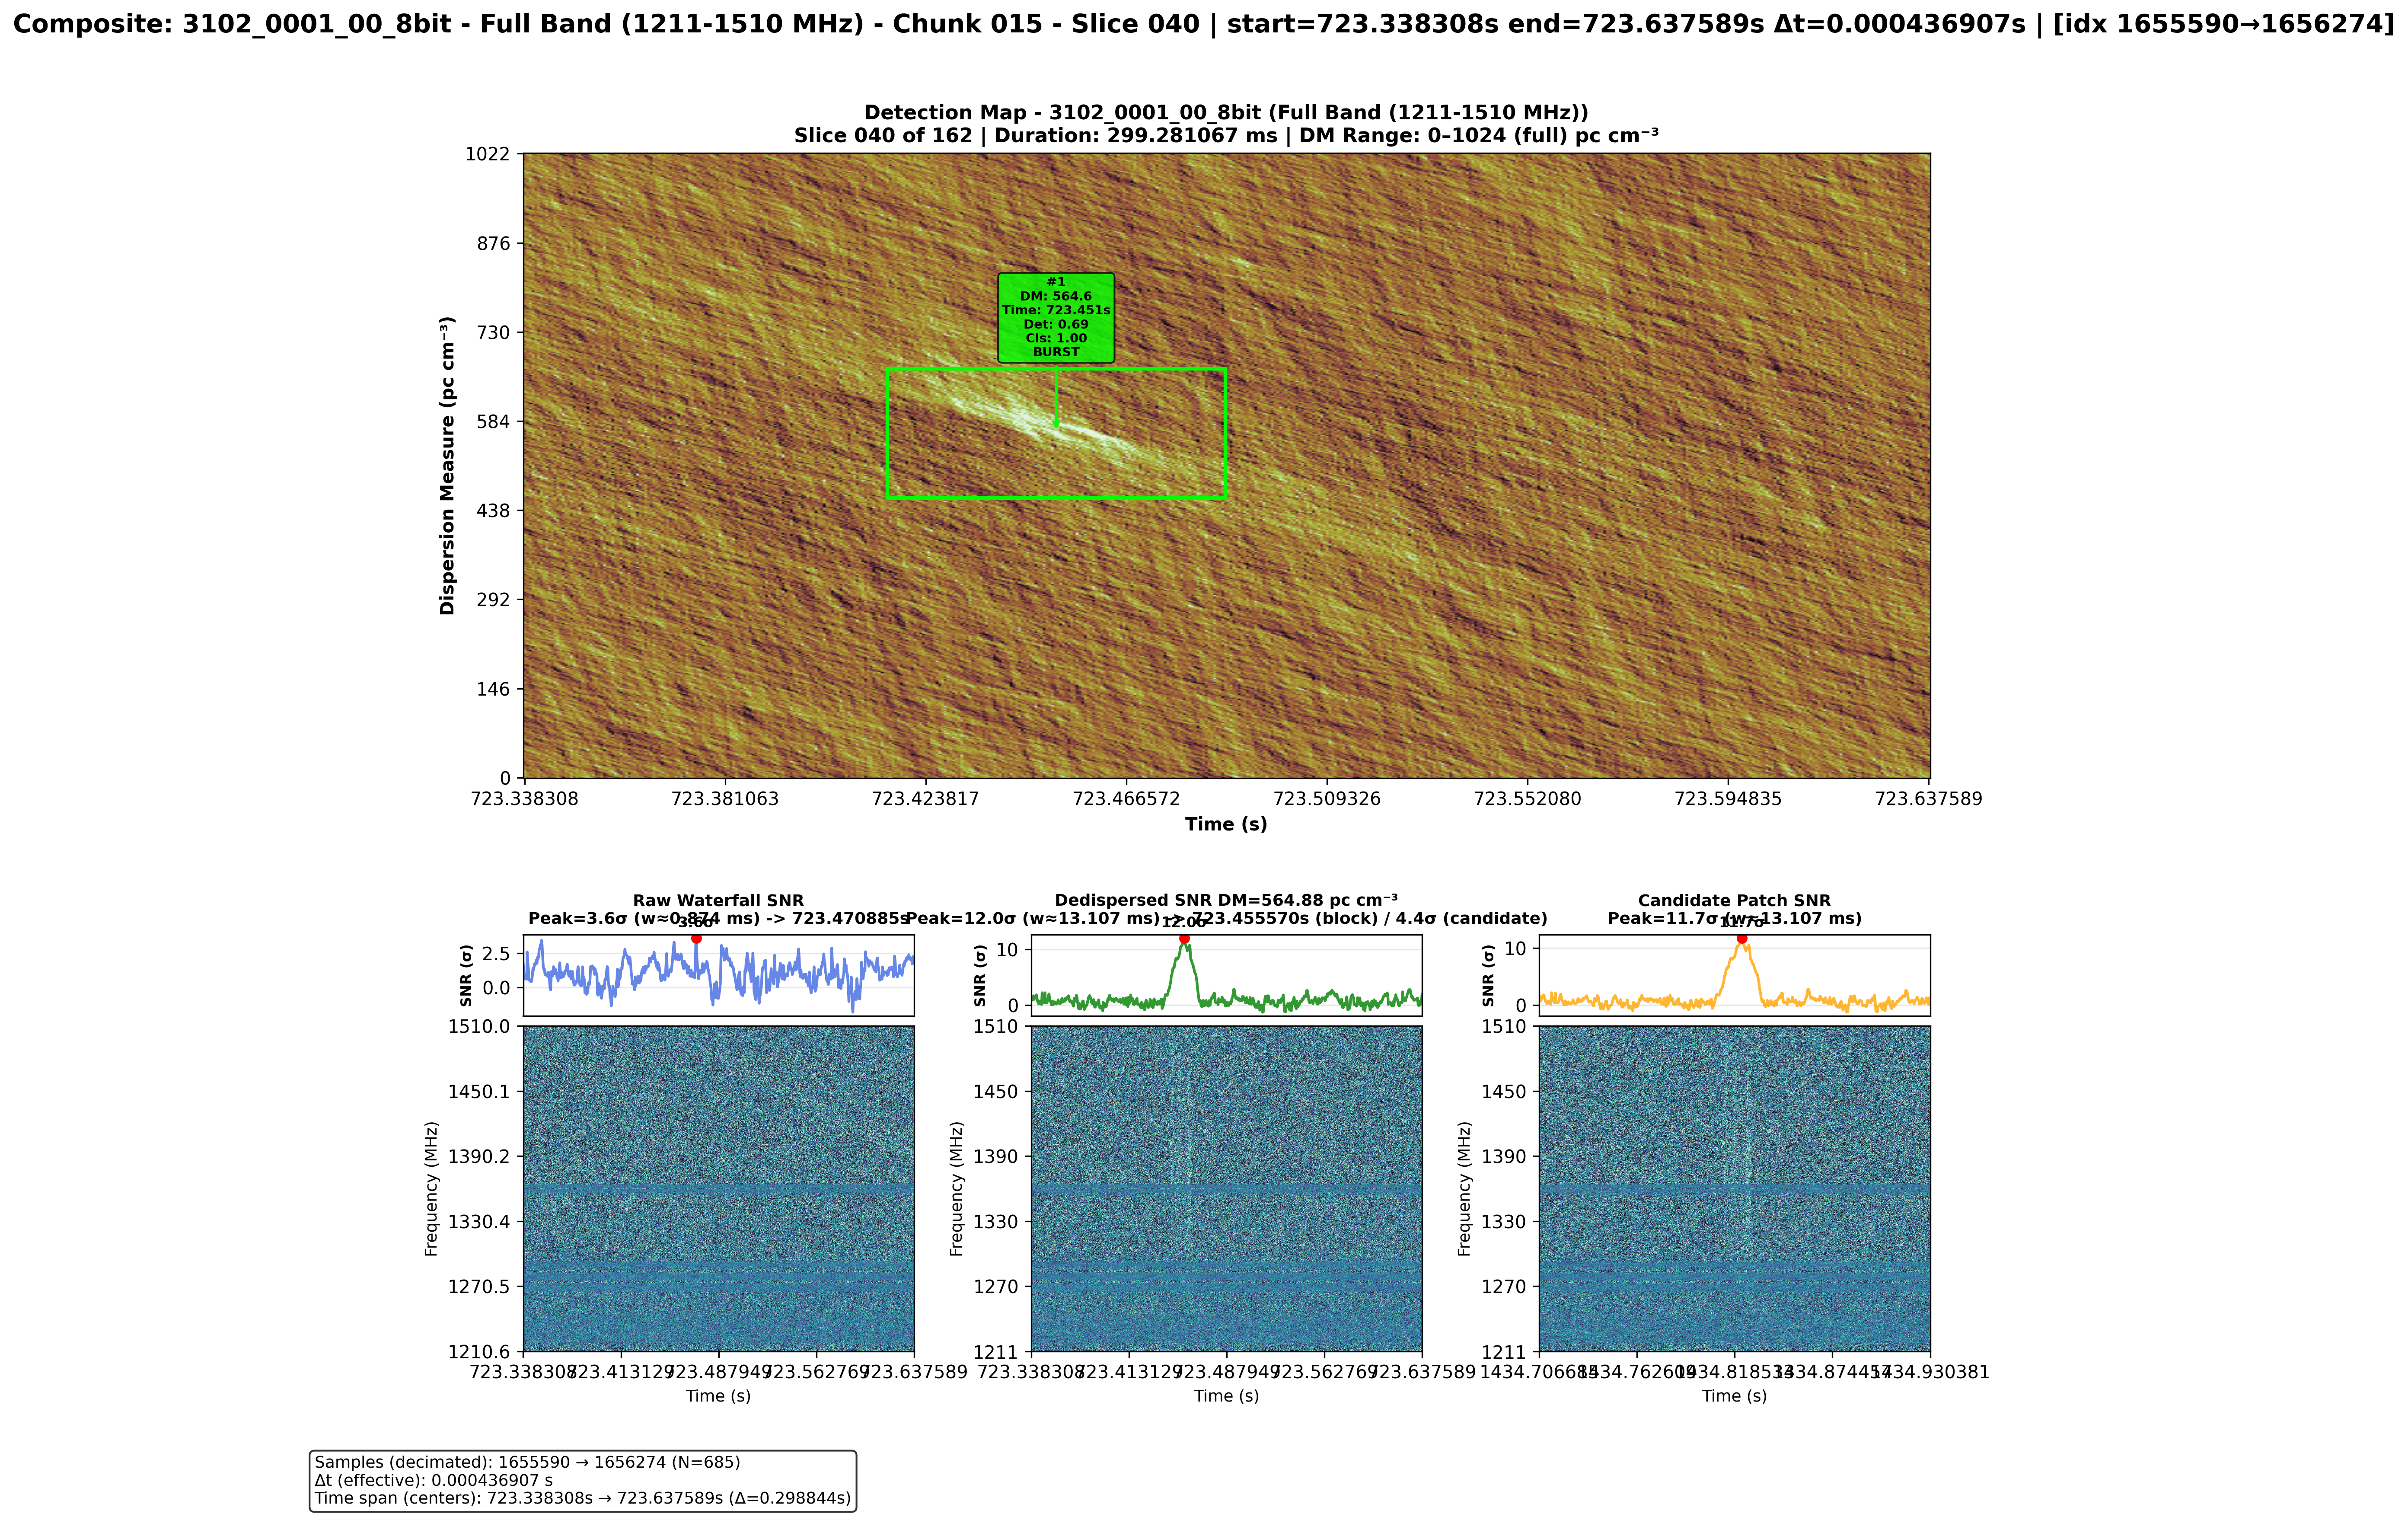
\includegraphics[width=\textwidth]{figures/Resultados/FRB121102/3102_0001_00_8bit_slice040.png}
    \caption[Descubrimiento científico: Segundo nuevo FRB 121102 - Complementaria]{Figura~\ref{fig:anexo_new_event_3102}. Segundo nuevo evento de FRB 121102 confirmado (Effelsberg, 1.4 GHz). Mapa DM-tiempo muestra detección en DM=564.88 pc cm$^{-3}$, t=723.5 s, SNR=12.0$\sigma$. Complementa la Figura~\ref{fig:new_event_3096} del Capítulo 5.}
    \label{fig:anexo_new_event_3102}
\end{figure}

\subsubsection{Figuras Complementarias - Línea 1 (Justificación)}

\begin{figure}[H]
    \centering
    \includegraphics[width=0.9\textwidth]{figures/Resultados/8 pulsos canonicos/2017-04-03-13_38_31_242_0005_t44.169_slice149.png}
    \caption[Justificación: Fallo Sistemático del Pipeline Clásico (Caso B, umbral conservador) - Complementaria]{Figura~\ref{fig:anexo_242_0005_slice149_highProb}. Fallo del pipeline clásico en alta frecuencia (ALMA, 86 GHz) con umbral conservador (DET\_PROB = 0.3). Mapa DM-tiempo muestra ausencia de detecciones para pulso confirmado en t=44.169 s. Complementa las Figuras~\ref{fig:142_0003_slice133_highProb} y~\ref{fig:142_0003_slice133_lowProb} del Capítulo 5.}
    \label{fig:anexo_242_0005_slice149_highProb}
\end{figure}

\begin{figure}[H]
    \centering
    \includegraphics[width=0.9\textwidth]{figures/DRAFTS-HF-Sin-Modificaciones/2017-04-03-13_38_31_242_0005_t44.169_slice149-lowProb.png}
    \caption[Justificación: Limitaciones Arquitecturales Irreductibles (Caso B, umbral sensible) - Complementaria]{Figura~\ref{fig:anexo_242_0005_slice149_lowProb}. Mismo pulso de la Figura~\ref{fig:anexo_242_0005_slice149_highProb} procesado con umbral sensible (DET\_PROB = 0.05). Mapa DM-tiempo muestra que el pulso permanece indetectable. Complementa las Figuras~\ref{fig:142_0003_slice133_highProb} y~\ref{fig:142_0003_slice133_lowProb} del Capítulo 5.}
    \label{fig:anexo_242_0005_slice149_lowProb}
\end{figure}

\subsubsection{Figuras Complementarias - Línea 2a (Solución Híbrida)}

\begin{figure}[H]
    \centering
    \includegraphics[width=0.95\textwidth]{figures/DRAFTS-HF-SNR/2017-04-03-12_56_05_230_0003_t36.548_slice121.png}
    \caption[Validación Línea 2a: Re-detección Exitosa de Pulso PRESTO - Complementaria]{Figura~\ref{fig:anexo_alma_presence_validation_1}. Re-detección de pulso PRESTO (ALMA, 86 GHz) mediante Línea 2a (matched filtering + ResNet18 en I). Mapa DM-tiempo muestra detección en t=36.548 s. Complementa la Figura~\ref{fig:alma_presence_validation_2} del Capítulo 5.}
    \label{fig:anexo_alma_presence_validation_1}
\end{figure}

\begin{figure}[H]
    \centering
    \includegraphics[width=0.95\textwidth]{figures/DRAFTS-HF-SNR/2017-04-03-08_16_13_0001_slice143.png}
    \caption[Descubrimiento Científico: Nuevo Pulso del Magnetar (Línea 2a) - Complementaria]{Figura~\ref{fig:anexo_alma_new_candidate_validation}. Nuevo candidato del magnetar PSR J1745-2900 (ALMA, 86 GHz) detectado por Línea 2a. Mapa DM-tiempo muestra detección en t=43.136 s, DM=46.9 pc cm$^{-3}$, score 1.00. Complementa los resultados de Línea 2a del Capítulo 5.}
    \label{fig:anexo_alma_new_candidate_validation}
\end{figure}

\begin{figure}[H]
    \centering
    \includegraphics[width=0.9\textwidth]{figures/Resultados/Pulsos ALMA SOLO DRAFTS/2017-04-03-12_47_05_0002_slice037.png}
    \caption[Capacidad de Resolución Temporal Fina: Continuación del Pulso Extendido (Slice 037) - Complementaria]{Figura~\ref{fig:anexo_slice037_multiple_detections}. Continuación del pulso extendido: 6 componentes adicionales en slice 037 (11.1-11.4 s). Mapa DM-tiempo muestra estructura temporal compleja. Complementa la Figura~\ref{fig:slice036_multiple_detections} del Capítulo 5, mostrando la secuencia completa de 13 componentes.}
    \label{fig:anexo_slice037_multiple_detections}
\end{figure}

\subsubsection{Figuras Complementarias - Línea 2b (Refinamiento Físico)}

\begin{figure}[H]
    \centering
    \includegraphics[width=0.95\textwidth]{figures/linea 2a/2017-04-03-08_16_13_0001_slice086.png}
    \caption[Deduplicación Inteligente mediante Clasificación Dual - Complementaria]{Figura~\ref{fig:anexo_linea2b_slice086_dedup}. Deduplicación de componentes temporales mediante clasificación dual I+L (Línea 2b, modo STRICT). Mapa DM-tiempo muestra dos candidatos cercanos; el sistema selecciona el de mayor coherencia polarimétrica. Complementa las Figuras~\ref{fig:linea2a_slice086} y~\ref{fig:linea2b_slice086_fp} del Capítulo 5.}
    \label{fig:anexo_linea2b_slice086_dedup}
\end{figure}

\begin{figure}[H]
    \centering
    \includegraphics[width=0.95\textwidth]{figures/linea 2a/2017-04-03-12_56_05_0001_slice102.png}
    \caption[Limitación de Especificidad: Múltiples Falsos Positivos Aceptados - Complementaria]{Figura~\ref{fig:anexo_linea2a_slice102}. Limitación de Línea 2a (solo I): slice 102 genera dos candidatos clasificados como BURST sin validación polarimétrica. Mapa DM-tiempo muestra falsos positivos aceptados. Complementa las Figuras~\ref{fig:linea2a_slice086} y~\ref{fig:linea2b_slice086_fp} del Capítulo 5.}
    \label{fig:anexo_linea2a_slice102}
\end{figure}

\begin{figure}[H]
    \centering
    \includegraphics[width=0.95\textwidth]{figures/linea 2a/2017-04-03-12_56_05_0001_slice102-FP.png}
    \caption[Éxito de Transfer Learning en Polarización: Filtrado Múltiple - Complementaria]{Figura~\ref{fig:anexo_linea2b_slice102_fp}. Éxito de Línea 2b (dual I+L): los mismos dos candidatos de la Figura~\ref{fig:anexo_linea2a_slice102} son rechazados tras clasificación dual. Mapa DM-tiempo muestra filtrado de falsos positivos. Complementa las Figuras~\ref{fig:linea2a_slice086} y~\ref{fig:linea2b_slice086_fp} del Capítulo 5.}
    \label{fig:anexo_linea2b_slice102_fp}
\end{figure}

\begin{figure}[H]
    \centering
    \includegraphics[width=0.95\textwidth]{figures/Resultados/Pulsos ALMA SOLO DRAFTS/2017-04-03-08_16_13_0002_slice101.png}
    \caption[Candidato Final Línea 2b: Coherencia Polarimétrica Validada (Candidato 2) - Complementaria]{Figura~\ref{fig:anexo_linea2b_candidate_2}. Candidato validado por clasificación dual I+L (Línea 2b, modo STRICT). Mapa DM-tiempo muestra pulso con clasificación BURST en ambas polarizaciones (archivo 08\_16\_13\_0002, slice 101). Complementa la Figura~\ref{fig:linea2b_candidate_1} del Capítulo 5.}
    \label{fig:anexo_linea2b_candidate_2}
\end{figure}

\begin{figure}[H]
    \centering
    \includegraphics[width=0.95\textwidth]{figures/Resultados/Pulsos ALMA SOLO DRAFTS/2017-04-03-12_47_05_0005_slice016.png}
    \caption[Candidato Final Línea 2b: Morfología Consistente (Candidato 3) - Complementaria]{Figura~\ref{fig:anexo_linea2b_candidate_3}. Candidato con morfología consistente en ambas polarizaciones (Línea 2b, modo STRICT). Mapa DM-tiempo muestra pulso clasificado como BURST en I+L (archivo 12\_47\_05\_0005, slice 016). Complementa la Figura~\ref{fig:linea2b_candidate_1} del Capítulo 5.}
    \label{fig:anexo_linea2b_candidate_3}
\end{figure}

\begin{figure}[H]
    \centering
    \includegraphics[width=0.95\textwidth]{figures/Resultados/Pulsos ALMA SOLO DRAFTS/2017-04-03-13_38_31_0003_slice081.png}
    \caption[Candidato Final Línea 2b: Coherencia Morfológica Polarimétrica (Candidato 4) - Complementaria]{Figura~\ref{fig:anexo_linea2b_candidate_4}. Candidato con coherencia morfológica polarimétrica validada (Línea 2b, modo STRICT). Mapa DM-tiempo muestra pulso clasificado como BURST en I+L (archivo 13\_38\_31\_0003, slice 081). Complementa la Figura~\ref{fig:linea2b_candidate_1} del Capítulo 5.}
    \label{fig:anexo_linea2b_candidate_4}
\end{figure}

\begin{figure}[H]
    \centering
    \fbox{\textit{[Figura de candidato 5 - Pendiente de generación]}}
    \caption[Línea 2b Candidato 5 - Complementaria]{Línea 2b Candidato 5: Pulso con clasificación BURST en I+L (modo STRICT). Pendiente de generación de figura y validación experta. Esta figura complementa la Figura~\ref{fig:linea2b_candidate_1} del Capítulo 5. \textit{Fuente: Elaboración propia}.}
    \label{fig:anexo_linea2b_candidate_5}
\end{figure}


\newpage
% Bibliografía estilo APA:
\bibliographystyle{plainnat}
\bibliography{bibliografia}

\end{document}
